\documentclass[12pt]{article}
\usepackage{graphicx} % Required for inserting images
\usepackage[left=25mm,right=25mm,top=25mm,bottom=25mm,paper=a4paper]{geometry} 
\usepackage{fancyhdr}
\usepackage{caption}
\usepackage{parskip}
\usepackage{fouriernc}
\usepackage{floatrow}
\usepackage{amsmath}
\usepackage{soul}
\usepackage{enumerate}
\usepackage{setspace} 
\usepackage{titlesec}
\usepackage{ragged2e}
\usepackage{changepage}
\usepackage{enumitem}
\usepackage{tocloft}


% Depth of numbering
\setcounter{secnumdepth}{4}
\setcounter{tocdepth}{4}
\setlength{\parindent}{0.5cm}
\setlength{\parskip}{12pt}

% Redefine the \paragraph command to act as a subsubsubsection
\makeatletter
\renewcommand{\paragraph}{%
 \@startsection{paragraph}{4}{\z@}%
 {-3.25ex plus -1ex minus -0.2ex}%
 {1.5ex plus 0.2ex}%
 {\normalfont\normalsize\bfseries}%
}
\makeatother

\begin{document}
\begin{spacing}{1.5}
\begin{adjustwidth}{0cm}{0cm}
\begin{justify}

\tableofcontents
\newpage
\listoffigures
\newpage
% \section{List of Figures And Tables}


\newpage
\pagestyle{fancy}
\renewcommand{\headruleskip}{5mm}
\renewcommand{\footruleskip}{10pt}
\renewcommand{\headrulewidth}{2pt}
\renewcommand{\footrulewidth}{4pt}
\fancyhead{}
\fancyhead [LO,CE]{NNM22AD017}
\fancyfoot{} % clear all footer fields
\fancyfoot[LE,RO]{\thepage}
\fancyfoot[LO,CE]{Cloud Computing Lab Manual}


\newpage
\section{Experiment 1}
Install Virtual box/VMware Workstation with different flavors of Linux or windows OS on top of windows7 or 8.
\subsection{Aim}
To Install VirtualBox/VMware Workstation with different flavors of Linux or windows OS on top of windows7 or 8.
\subsection{Procedure}

\textbf{Step 1:} \\
Open the VirtualBox website by going to https://www.virtualbox.org/ in your Internet browser. This is where you’ll download the VirtualBox setup file.

\textbf{Step 2:} \\
Click the "Download VirtualBox" button, which is located in the middle of the page. This will take you to the downloads page.

\begin{figure}[H]
    \centering
    \includegraphics[width=1.0\textwidth]{exp 1/Screenshot 2024-11-11 135055.png}
    \caption{Official website of VM VirtualBox}
    \label{fig: 1}
\end{figure}

\textbf{STEP 3:} \\
Click windows host. You'll see this link below the "VirtualBox 5.2.8 platform packages” heading. The VirtualBox EXE file will begin downloading onto your computer.

\textbf{STEP 4:} \\
Open the VirtualBox EXE file. Go to the location where the EXE file was downloaded and double-click the file. This will open the VirtualBox installation window. 
Navigate through the installation prompts by doing the following:

\begin{itemize}
    \item Click \textbf{Next} on the first three pages.
    \item Click \textbf{Yes} when prompted.
    \item Click \textbf{Install}.
    \item Click \textbf{Yes} when prompted.
    \item Click \textbf{Install} when prompted. This will start the installation of VirtualBox on your computer.
    \item Click \textbf{Finish} when prompted. This button is in the lower-right side of the window and will close the installation window, opening VirtualBox.
\end{itemize}

\begin{figure}[H]
    \centering
    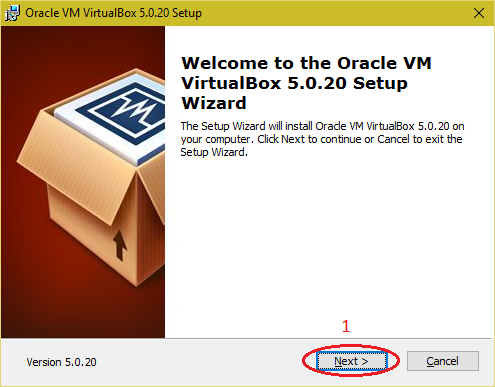
\includegraphics[width=0.6\textwidth]{exp 1/vbox001.png}
    \caption{VirtualBox Setup}
    \label{fig: 1}
\end{figure}

\begin{figure}[H]
    \centering
    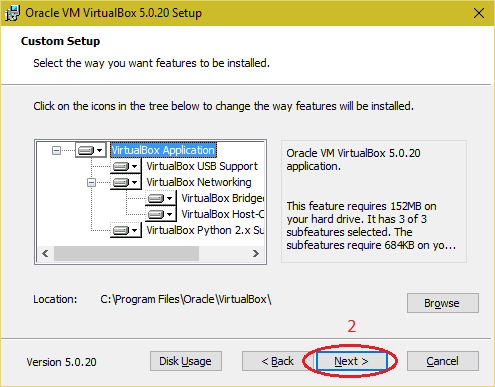
\includegraphics[width=0.7\textwidth]{exp 1/vbox002.png}
    \caption{VirtualBox Custom Setup}
    \label{fig: 1}
\end{figure}

\begin{figure}[H]
    \centering
    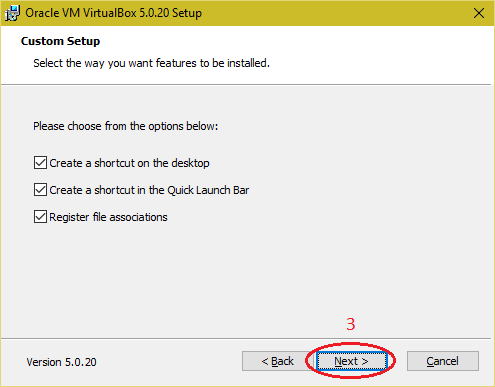
\includegraphics[width=0.7\textwidth]{exp 1/vbox003.png}
    \caption{VirtualBox Setup}
    \label{fig: 1}
\end{figure}

\begin{figure}[H]
    \centering
    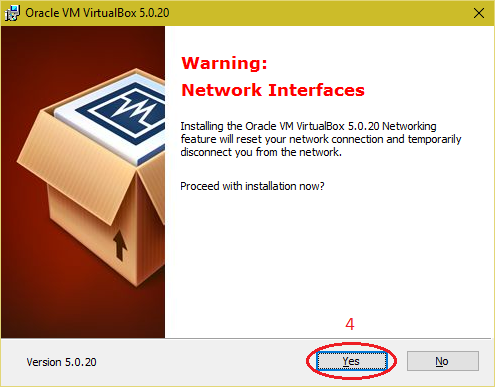
\includegraphics[width=0.7\textwidth]{exp 1/vbox004.png}
    \caption{VirtualBox Setup}
    \label{fig: 1}
\end{figure}

\begin{figure}[H]
    \centering
    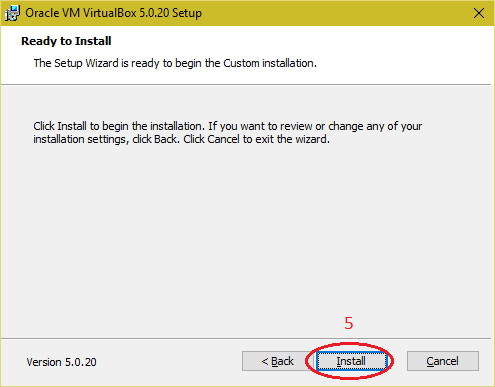
\includegraphics[width=0.7\textwidth]{exp 1/vbox005.png}
    \caption{VirtualBox Setup}
    \label{fig: 1}
\end{figure}


\textbf{STEP 5:} \\
Open Oracle VM VirtualBox Manager, Type a name for the new virtual machine. (Ubuntu), I'll enter 'ubuntu6969'. Note that VirtualBox automatically changes 'Type' to Linux and 'Version' to 'Ubuntu (64 bit)'. These two options are exactly what we need

\begin{figure}[H]
    \centering
    \includegraphics[width=0.8\textwidth]{exp 1/Screenshot 2024-11-11 141414.png}
    \caption{Creation of VM}
    \label{fig: 1}
\end{figure}

\textbf{STEP 6:} \\
The memory size depends on your host machine memory size and select the size of the virtual hard disk and click ‘next’ button. \\
Note that VirtualBox will create a swap partition with the same amount space as base memory you have entered here. So later when you are selecting the size of the virtual hard drive, make sure it is large enough since the hard drive will be splitted into root (/)and swap partitions. The root partition contains by default all your system files, program settings and documents.

\begin{figure}[H]
    \centering
    \includegraphics[width=0.8\textwidth]{exp 1/Screenshot 2024-11-11 141453.png}
    \caption{Configuration of Hardware}
    \label{fig: 1}
\end{figure}

\begin{figure}[H]
    \centering
    \includegraphics[width=0.8\textwidth]{exp 1/Screenshot 2024-11-11 141504.png}
    \caption{Configuration of Virtual HardDisk}
    \label{fig: 1}
\end{figure}

\textbf{STEP 7:} \\
Select the created Virtual machine and click ‘start’ button.

\begin{figure}[H]
    \centering
    \includegraphics[width=0.9\textwidth]{exp 1/Screenshot 2024-11-11 141518.png}
    \caption{Starting the VM}
    \label{fig: 1}
\end{figure}

Install Ubuntu 

Now you shall see a 'Welcome' screen. Click 'Install Ubuntu' button. Note that the installation process may differ a little bit from version to version

\begin{figure}[H]
    \centering
    \includegraphics[width=0.9\textwidth]{exp 1/Screenshot 2024-11-11 141844.png}
    \caption{Installing Ubuntu}
    \label{fig: 1}
\end{figure}

\begin{figure}[H]
    \centering
    \includegraphics[width=0.9\textwidth]{exp 1/Screenshot 2024-11-13 at 11.07.06 PM.png}
    \caption{Selecting the software language}
    \label{fig: 1}
\end{figure}

\textbf{STEP 8:} \\
Click continue and make sure 'Erase disk and install Ubuntu' option is selected and click 'Install Now'

\begin{figure}[H]
    \centering
    \includegraphics[width=0.9\textwidth]{exp 1/Screenshot 2024-11-13 at 11.08.32 PM.png}
    \caption{Installation Type}
    \label{fig: 1}
\end{figure}

\textbf{STEP 9:} \\
Ubuntu will ask you a few questions. If the default is good, click 'Continue', then we need to fill the username and password. \\
Note that this user will have root/sudo privilege. Click 'Continue' button

\begin{figure}[H]
    \centering
    \includegraphics[width=0.9\textwidth]{exp 1/Screenshot 2024-11-13 at 11.09.53 PM.png}
    \caption{Username and Password }
    \label{fig: 1}
\end{figure}

\textbf{STEP 10:} \\
After installation is complete, click 'Restart Now' button. When you see a screen with a black background saying 'Please remove installation media and close the tray (if any) then press ENTER

\begin{figure}[H]
    \centering
    \includegraphics[width=0.9\textwidth]{exp 1/Screenshot 2024-11-11 142120.png}
    \caption{Setting up Ubuntu}
    \label{fig: 1}
\end{figure}

\begin{figure}[H]
    \centering
    \includegraphics[width=0.9\textwidth]{exp 1/Screenshot 2024-11-11 142133.png}
    \caption{Ubuntu homepage}
    \label{fig: 1}
\end{figure}

\subsection{Result}
Thus the installation of a virtual machine using Virtualbox/VMware Workstation on top of windows7 or 8 is done successfully.

\newpage


\section{Experiment 2}
Install a C compiler in the virtual machine created using VirtualBox and execute simple programs.

\subsection{Aim}
To find the procedure to install a C Compiler in the Virtual Machine and execute a C program.

\subsection{Procedure}

\textbf{STEP 1:} \\
Open the Virtual Machine, Start your Ubuntu virtual machine from Virtual-
Box.

\textbf{STEP 2:} \\
Update System Packages: Once Ubuntu loads, open the Terminal

\begin{figure}[H]
    \centering
    \includegraphics[width=0.8\textwidth]{exp 2/Picture 1.png}
    \caption{VM (Ubuntu) terminal}
    \label{fig: 1}
\end{figure}

Enter the following command to update the system packages:
\begin{center}
\parbox{\textwidth}{
\centering
\texttt{sudo apt update} \\
\texttt {sudo apt upgrade}
}
\end{center}

\textbf{STEP 3:} \\
INSTALLATION OF C COMPILER: In the terminal, install the required build essentials, including the GCC (GNU Compiler Collection) C compiler

\begin{center}
\parbox{\textwidth}{
\centering
\texttt{Sudo apt install gcc} \\
\texttt{Sudo apt install  build-essential}
}
\end{center}

\begin{figure}[H]
    \centering
    \includegraphics[width=0.8\textwidth]{exp 2/Picture 2.png}
    \caption{sudo apt install build-essential}
    \label{fig: 1}
\end{figure}

\begin{figure}[H]
    \centering
    \includegraphics[width=0.8\textwidth]{exp 2/Screenshot 2024-11-13 at 11.29.45 PM.png}
    \caption{gcc --version }
    \label{fig: 1}
\end{figure}


\textbf{STEP 4:} \\
After the compiler is installed, create a new C program file.
In the terminal, run:
\begin{center}
\parbox{\textwidth}{
\centering
\texttt{touch hello.c}
}
\end{center}

This will open the editor. Write the following C code for the "Hello, World!" program:

\begin{center}
\begin{verbatim}
#include <stdio.h>

int main() {
    printf("Hello, World!\n");
    return 0;
}
\end{verbatim}
\end{center}

Save the file as \texttt{hello.c}.


\textbf{STEP 5:} \\
Compile and Execute the Program C Program: \\
Now, compile the program using the \texttt{gcc} compiler. In the terminal, run:

\begin{center}
\texttt{gcc hello.c -o hello}
\end{center}

After the compilation is successful, execute the program:

\begin{center}
\texttt{./hello}
\end{center}

The output \texttt{Hello, World!} will be printed on the terminal.


\begin{figure}[H]
    \centering
    \includegraphics[width=0.8\textwidth]{exp 2/Screenshot 2024-11-13 at 11.31.58 PM.png}
    \caption{Hello World program in C}
    \label{fig: 1}
\end{figure}




\subsection{Result}
Thus the C Compiler is installed successfully and executed a sample C program.




\newpage

\section{Experiment 3}
Discuss bare metal hypervisor and Hosted hypervisor and list a few of them with detailed
explanation.
\subsection{Bare-Metal Hypervisor}
A Type 1 hypervisor, commonly referred to as a \textbf{bare-metal hypervisor}, represents a sophisticated virtualization framework that interfaces directly with the system's physical hardware infrastructure. As a primary control layer, it orchestrates both the underlying hardware resources and the multiple guest operating systems operating above it. By eliminating intermediary layers, this direct hardware interaction enables superior performance metrics compared to alternative virtualization approaches.

In contrast, Type 2 hypervisors, known as \textbf{hosted hypervisors}, operate within the ecosystem of a conventional operating system. This architectural design introduces an additional abstraction layer, as all hardware communications must traverse through the host operating system. The consequence of this layered structure manifests in heightened latency within the virtual machine environments, as each instruction must navigate through the host OS before reaching the physical hardware.

\subsection{Advantages of Bare-Metal Hypervisors}
\begin{itemize}
    \item Resource management efficiency
    \item System performance optimization
    \item Hardware utilization patterns
    \item Overall virtualization overhead
\end{itemize}

\subsection{Top Bare-Metal Hypervisors}
There are several popular bare-metal hypervisors, both commercial and open-source. Some of the most well-known options include:

\begin{enumerate}
    \item Kernel-based Virtual Machine (KVM)
    \item Microsoft Hyper-V
    \item Oracle VM Server for x86
    \item VMware ESXi
    \item Xen Project
    \item RedHat Virtualization
\end{enumerate}

\subsection{Overview of Popular Bare-Metal Hypervisors}

\textbf{KVM (Kernel-based Virtual Machine)} \\
KVM (Kernel-based Virtual Machine) represents a unique hybrid hypervisor architecture that combines aspects of both Type 1 and Type 2 virtualization. While it leverages direct hardware virtualization capabilities like a bare-metal hypervisor.

\textbf{Microsoft Hyper-V} \\
Hyper-V is a Type 1 hypervisor that runs directly on hardware. It offers excellent
resource allocation for VMs, such as dynamic memory adjustments.

\textbf{VMware ESXi} \\
VMware ESXi is a lightweight, Type 1 hypervisor with a small footprint of only
150MB.

\subsection{Hosted Hypervisors}
Hosted hypervisors (Type 2) run on top of an existing operating system. Some popular
hosted hypervisors include:
\begin{enumerate}
    \item VirtualBox
    \item QEMU
    \item Parallels Desktop
    \item VMware Workstation Pro
\end{enumerate}

\textbf{VirtualBox} \\
Oracle VM VirtualBox is a versatile, free, and open-source hosted hypervisor that functions across multiple platforms including Windows, Linux, macOS, and Solaris. It offers comprehensive virtualization features including support for diverse guest operating systems, snapshot management for system state preservation, live VM migration capabilities, advanced networking configurations (NAT, bridged, host-only), and seamless file sharing between host and guest systems. The platform enhances user experience through features like seamless mode integration, multi-monitor support, and cross-platform compatibility, while the VirtualBox Extension Pack provides additional functionality such as USB device support and remote desktop capabilities. For advanced users and automation needs, VirtualBox includes a robust command-line interface (VBoxManage) alongside its traditional GUI, making it an ideal choice for both personal and professional virtualization requirements, particularly among developers and system administrators requiring local virtual environments.

\textbf{QEMU} \\
QEMU (Quick Emulator) operates as a Type 2 hypervisor that employs dynamic binary translation for processor emulation, particularly effective when integrated with KVM for enhanced performance. It excels in supporting multiple CPU architectures (x86, ARM, PowerPC, MIPS, SPARC), making it invaluable for cross-platform virtualization needs. The platform offers comprehensive features including snapshot management, network emulation capabilities, and extensive disk and device emulation support. QEMU's versatility makes it particularly useful in testing and development environments, especially when actual hardware access is limited. When combined with KVM, it achieves notable performance improvements through hardware acceleration, while maintaining its robust capabilities for complex network configurations and storage device emulation, making it a comprehensive solution for both development and production environments.

\textbf{Parallels Desktop} \\
Parallels Desktop is a sophisticated hosted hypervisor, officially sanctioned by Microsoft for running Windows on Apple Silicon processors (M1, M2), that offers seamless integration between macOS and Windows environments. It combines robust security features including VM encryption and multi-factor authentication with advanced capabilities such as cloud integration (Azure, AWS), GPU acceleration, and DirectX/OpenGL support. The platform's standout features include Coherence Mode for native-like Windows application execution, comprehensive VM configuration options, and optimized performance for resource-intensive applications. With seamless macOS integration supporting features like Time Machine backup and Retina display compatibility, along with efficient cross-platform functionality, Parallels Desktop delivers a high-performance virtualization solution particularly suited for both individual users and enterprises requiring sophisticated graphics capabilities and development environments on Apple hardware.

\textbf{VMware Workstation Pro} \\
VMware Workstation Pro is a powerful hosted hypervisor designed for creating and managing virtual machines (VMs) on Windows and Linux systems, catering primarily to developers, IT professionals, and system administrators. It features cloning capabilities, allowing users to quickly create linked or full clones of VMs for testing or deployment purposes. The remote management functionality enables control over local and remote VMs via vCenter and ESXi hosts, enhancing operational flexibility. Security is prioritized through encryption, safeguarding sensitive data within VMs, which is crucial for compliance with security policies. Users can utilize snapshot functionality to save and restore VM states, facilitating error recovery and configuration management. Advanced network simulation capabilities allow for the creation of isolated networks for testing without impacting the host system, while virtual networking options enable custom network setups with NAT and bridged connections. VMware Workstation Pro supports a wide array of operating systems, optimizing resource allocation for CPU, memory, and disk space according to user needs. Additionally, it integrates seamlessly with VMware vSphere, allowing for the migration of VMs between environments, thus providing a robust hybrid cloud experience.

\newpage

\section{Experiment 4}
To demonstrates application-level virtualization 
\subsection{Aim} 
To demonstrates application-level virtualization by installing and using
Notepad++ on a Linux system via Wine, which allows running Windows applications
on Linux.
\subsection{Procedure}

\textbf{STEP 1:} \\
Ensure Wine is Installed in the System, To install Wine on a Linux system, open a terminal and run the following command:



\begin{center}
\texttt{sudo apt update}
\end{center}
\begin{center}
\texttt{sudo apt install wine64}
\end{center}

\begin{figure}[H]
    \centering
    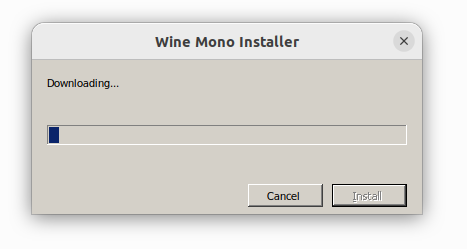
\includegraphics[width=0.9\textwidth]{exp 4/image.png}
    \caption{Installer}
    \label{fig: 1}
\end{figure}

\textbf{STEP 2:} \\
Download the Notepad++ Installer: Visit the official Notepad++ website to download the installer for Linux systems using Wine.

\begin{figure}[H]
    \centering
    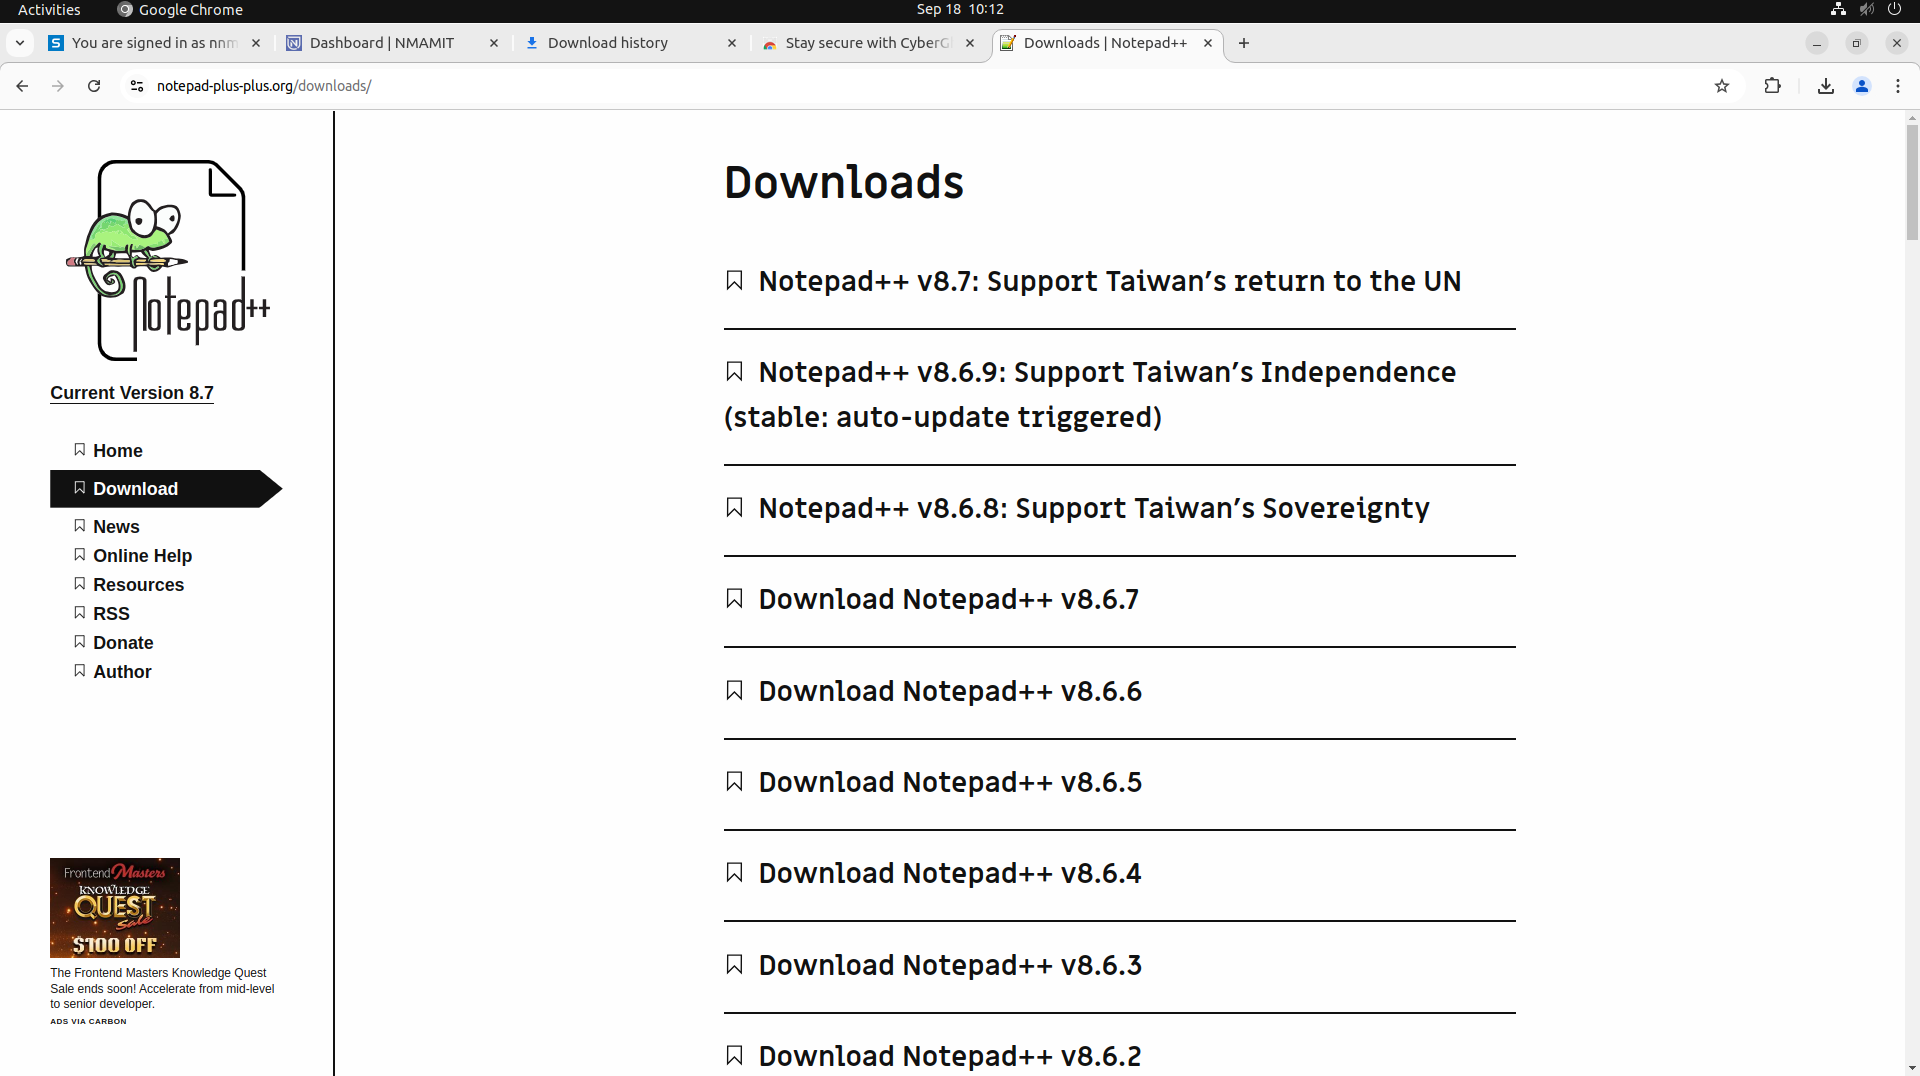
\includegraphics[width=0.9\textwidth]{exp 4/Screenshot from 2024-09-18 10-12-51.png}
    \caption{Official website of Notepad++}
    \label{fig: 1}
\end{figure}

\textbf{STEP 3:} \\
Select Wine as the Application to Run the Installer: In the context menu, select Open With Wine or Run with Wine

\begin{figure}[H]
    \centering
    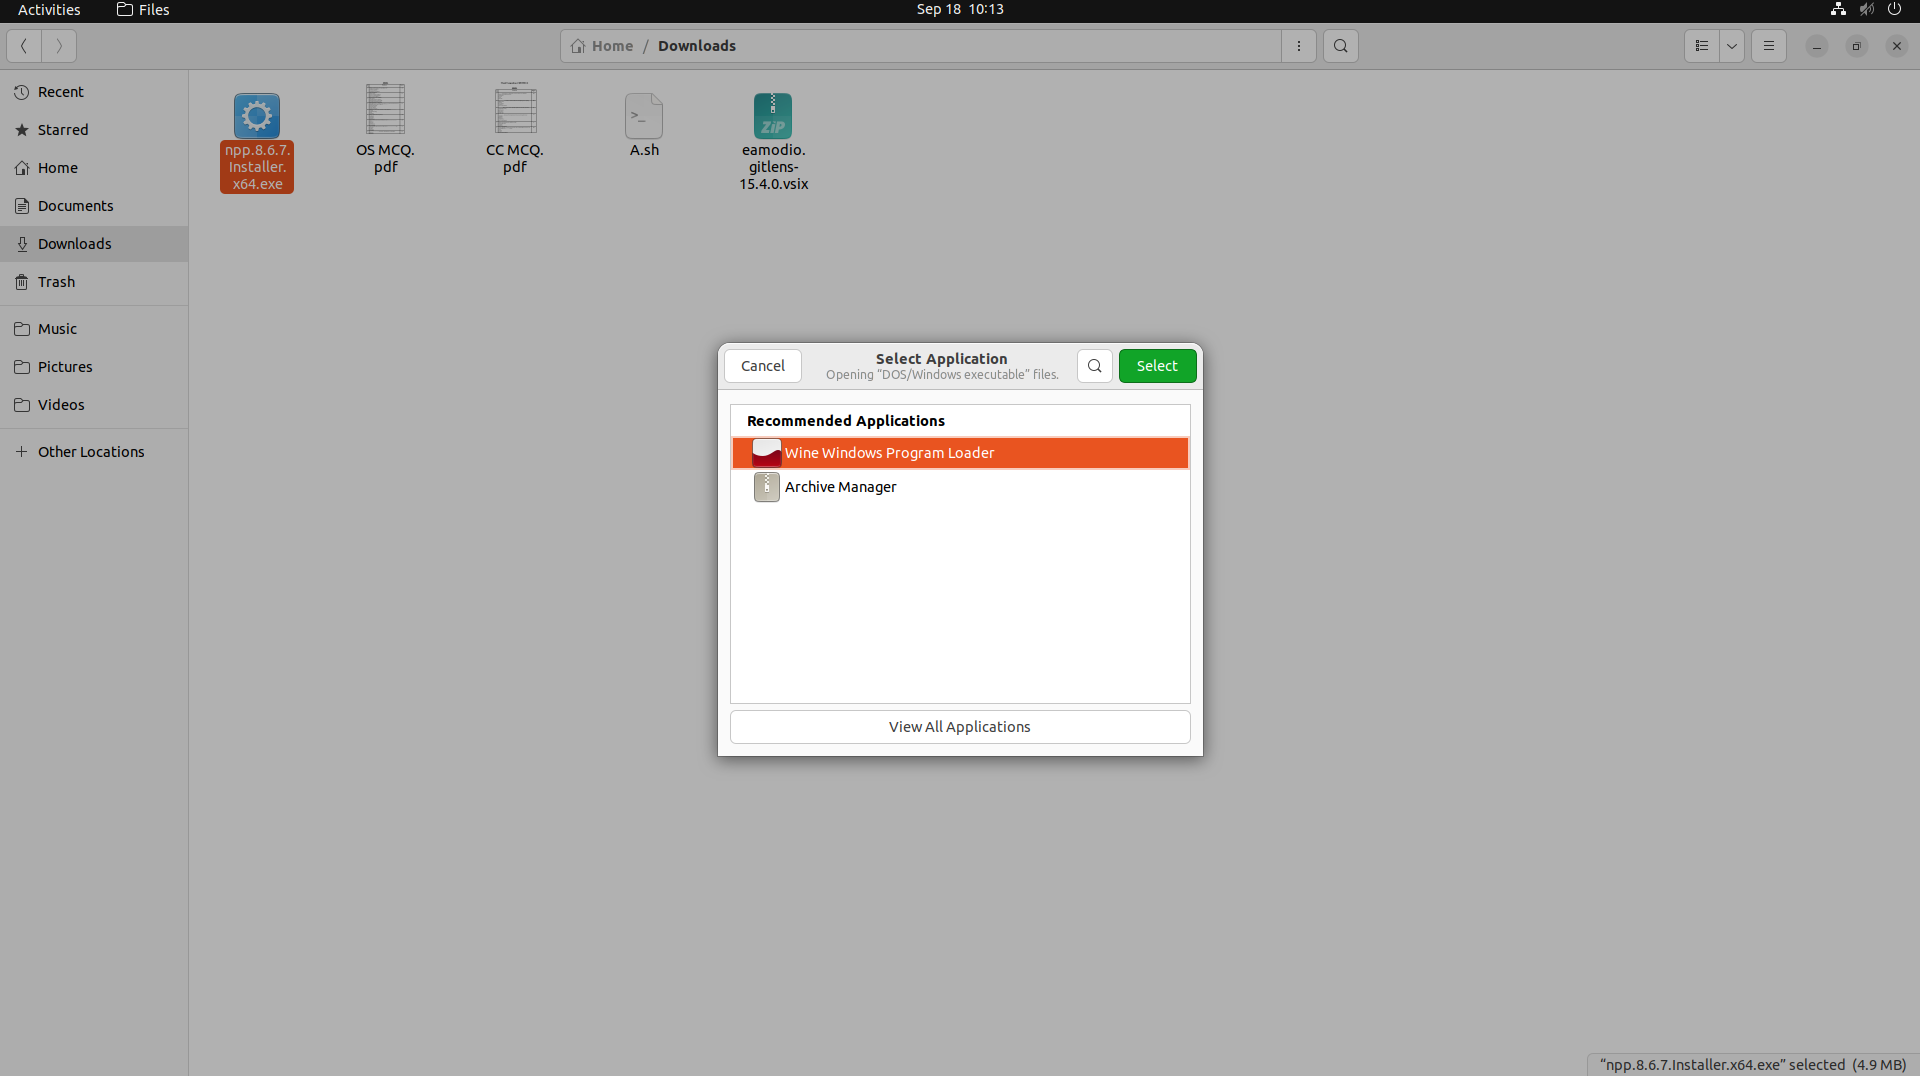
\includegraphics[width=0.9\textwidth]{exp 4/Screenshot from 2024-09-18 10-13-20.png}
    \caption{select WINE application}
    \label{fig: 1}
\end{figure}

\textbf{STEP 4:} \\
Follow the Instructions in the Notepad++ Installation Wizard: During the Wine application launch, the Notepad++ installation wizard will initiate automatically. To proceed with the installation, click "I Agree" to accept the terms and conditions, then choose your preferred installation directory - either opt for the default Wine directory or specify a custom location of your choice.

\begin{figure}[H]
    \centering
    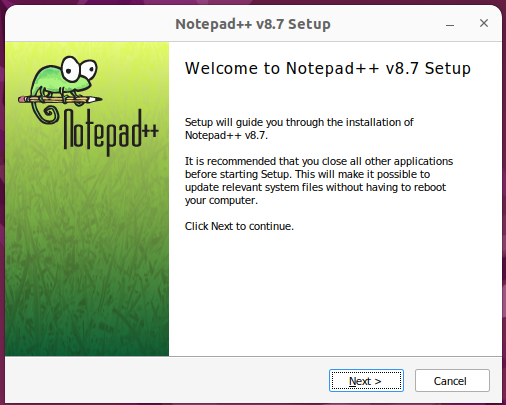
\includegraphics[width=0.7\textwidth]{exp 4/image1.png}
    \caption{Notepad++ Setup }
    \label{fig: 1}
\end{figure}

\begin{figure}[H]
    \centering
    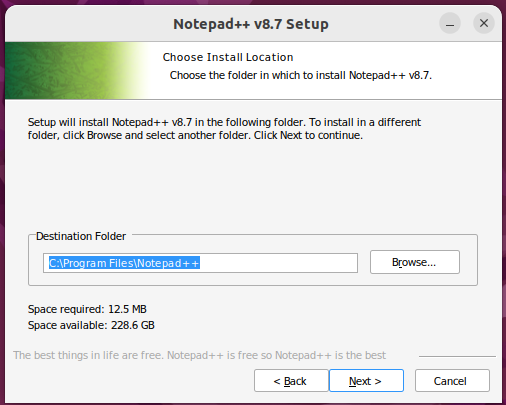
\includegraphics[width=0.7\textwidth]{exp 4/image2.png}
    \caption{Notepad++ Setup Wizard }
    \label{fig: 1}
\end{figure}

\textbf{STEP 5:} \\
Click Install and Finish the Setup: After confirming all installation settings, click Install to begin the process. Once the installation is complete, click Finish to exit the installer.

\begin{figure}[H]
    \centering
    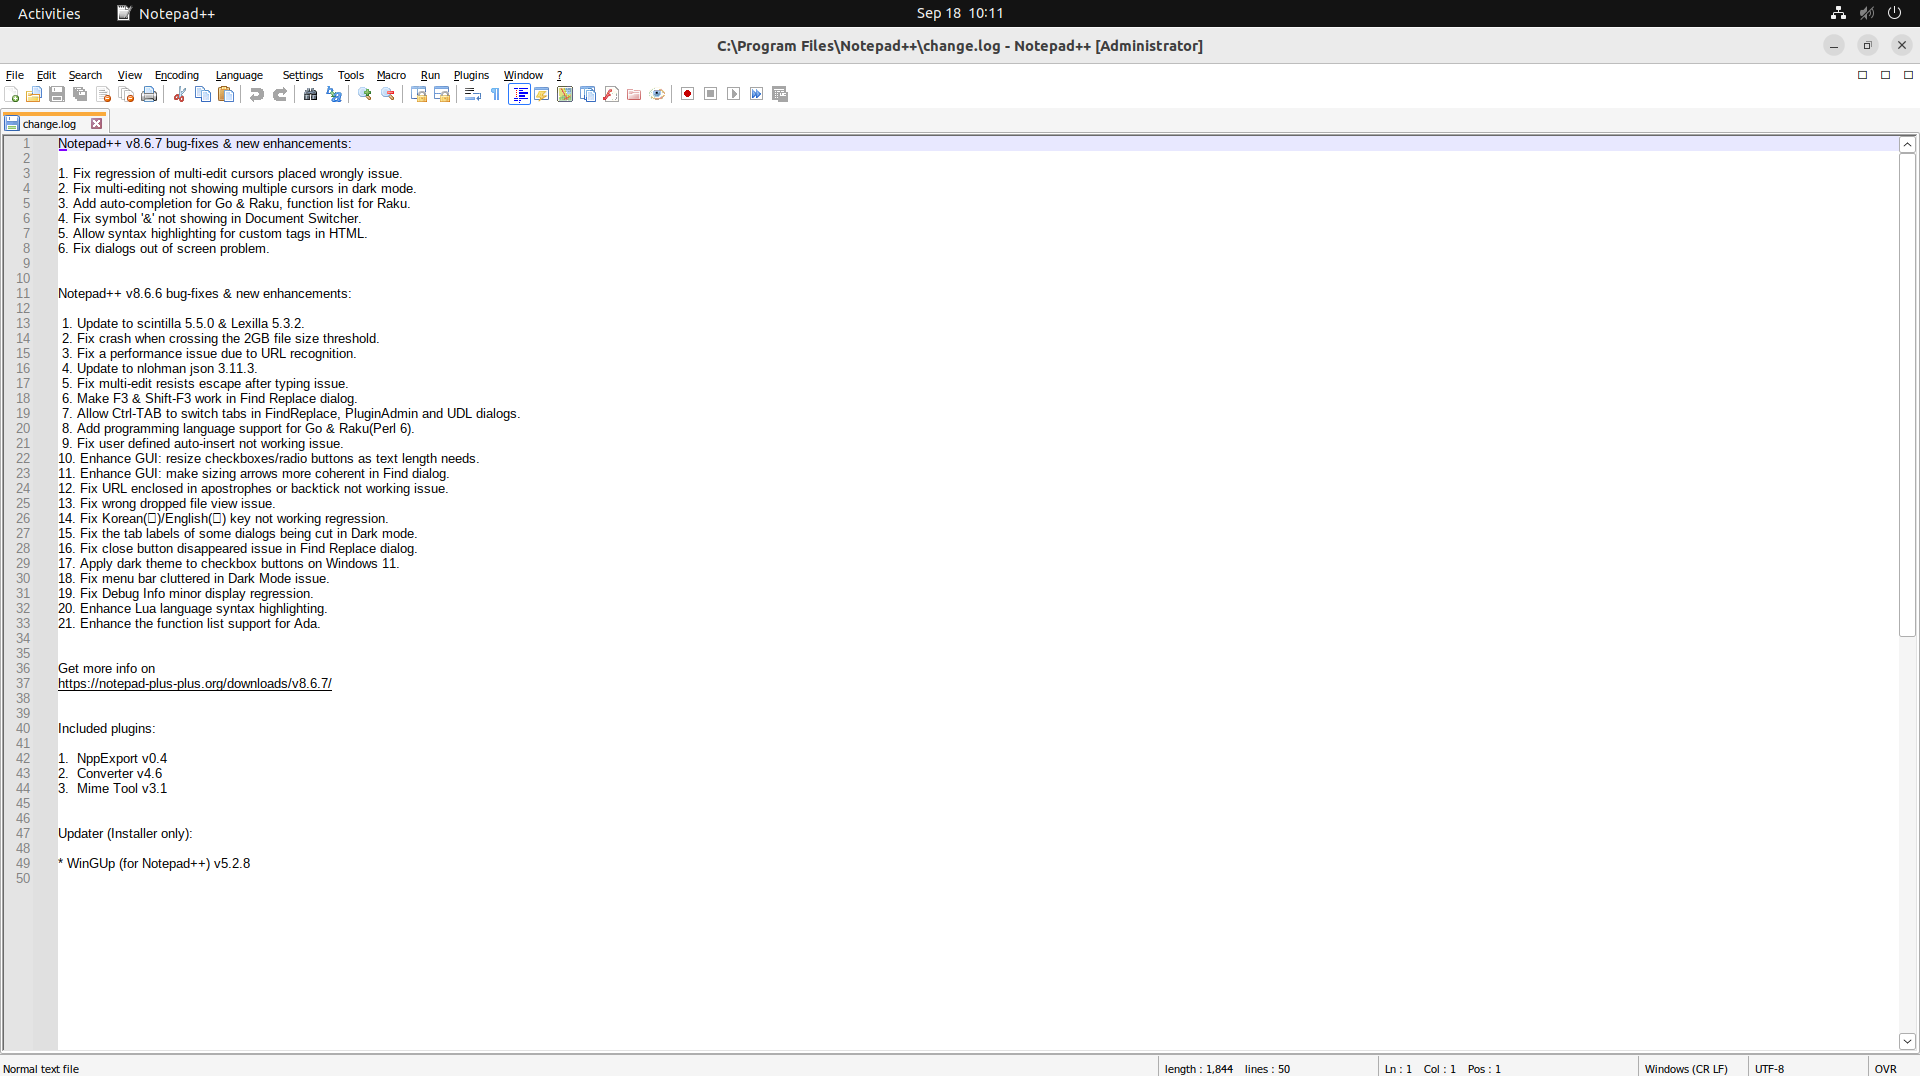
\includegraphics[width=0.9\textwidth]{exp 4/Screenshot from 2024-09-18 10-11-28.png}
    \caption{First view of Notepad++}
    \label{fig: 1}
\end{figure}

\textbf{STEP 6:} \\
Create and Save a New Text File in Notepad++: When Notepad++ launches, create a new text file by selecting File→New from the menu. Enter your desired text content. Once you've added the content, save your work by clicking File→Save As and choose your preferred storage location for the file.

\begin{figure}[H]
    \centering
    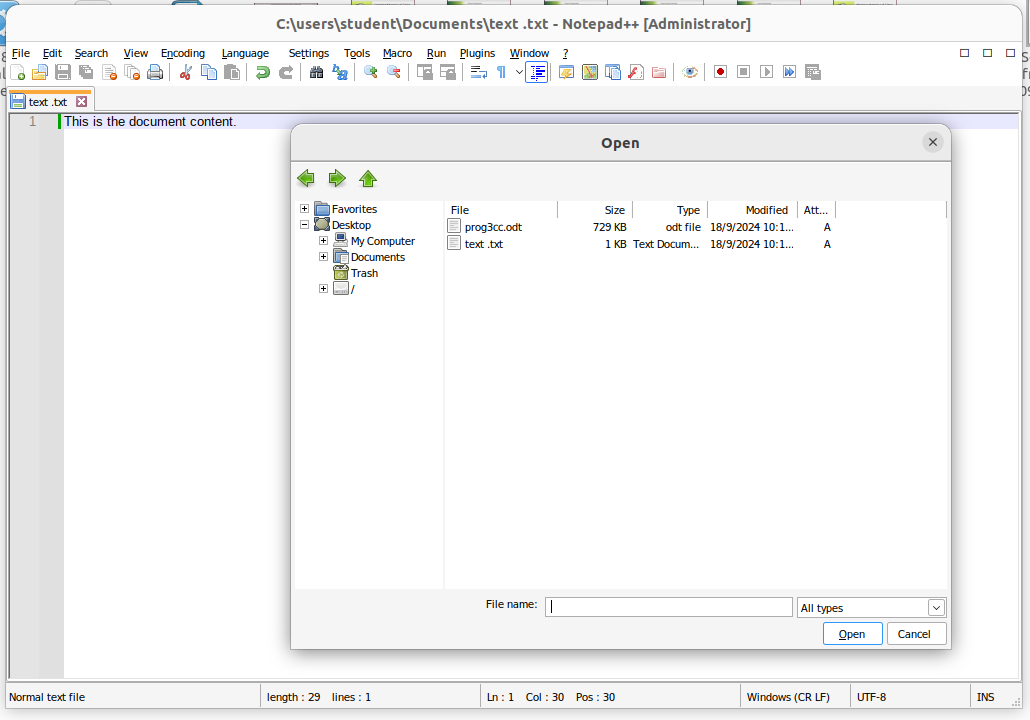
\includegraphics[width=0.9\textwidth]{exp 4/image3.png}
    \caption{Creating and saving the new file}
    \label{fig: 1}
\end{figure}

\subsection{Result} 
In this experiment we successfully demonstrated application-level virtualization by running Notepad++ (a Windows application) efficiently on a Linux system through Wine, proving cross-platform compatibility without requiring native Windows OS installation.

\newpage

\section{Experiment 5}
Demonstrating and Implementing PaaS to Deploy a Simple Web Application

\subsection{Aim}
To Demonstrate and Implementing PaaS to Deploy a Simple Web Application

\subsection{Procedure}

\textbf{Prerequisites}

\begin{itemize}
    \item \textbf{Google Cloud Account:} Ensure that you have a Google Cloud Account.
    \item \textbf{Google Cloud SDK:} Install the Google SDK on your machine to manage GCP resources from the command line.
\end{itemize}

To deploy a simple ”Hello World” application using Platform as a Service (PaaS)
on Google Cloud Platform (GCP), we will use Google App Engine with a Node.js
application. The steps are as follows:

\textbf{STEP 1:} \\
To begin with Google Cloud deployment, access the Google Cloud Console, create a new project by selecting "New Project" from the project dropdown menu, assign a project name while noting down the Project ID for future reference, and ensure billing is activated for the project to enable deployment capabilities.

\begin{figure}[H]
    \centering
    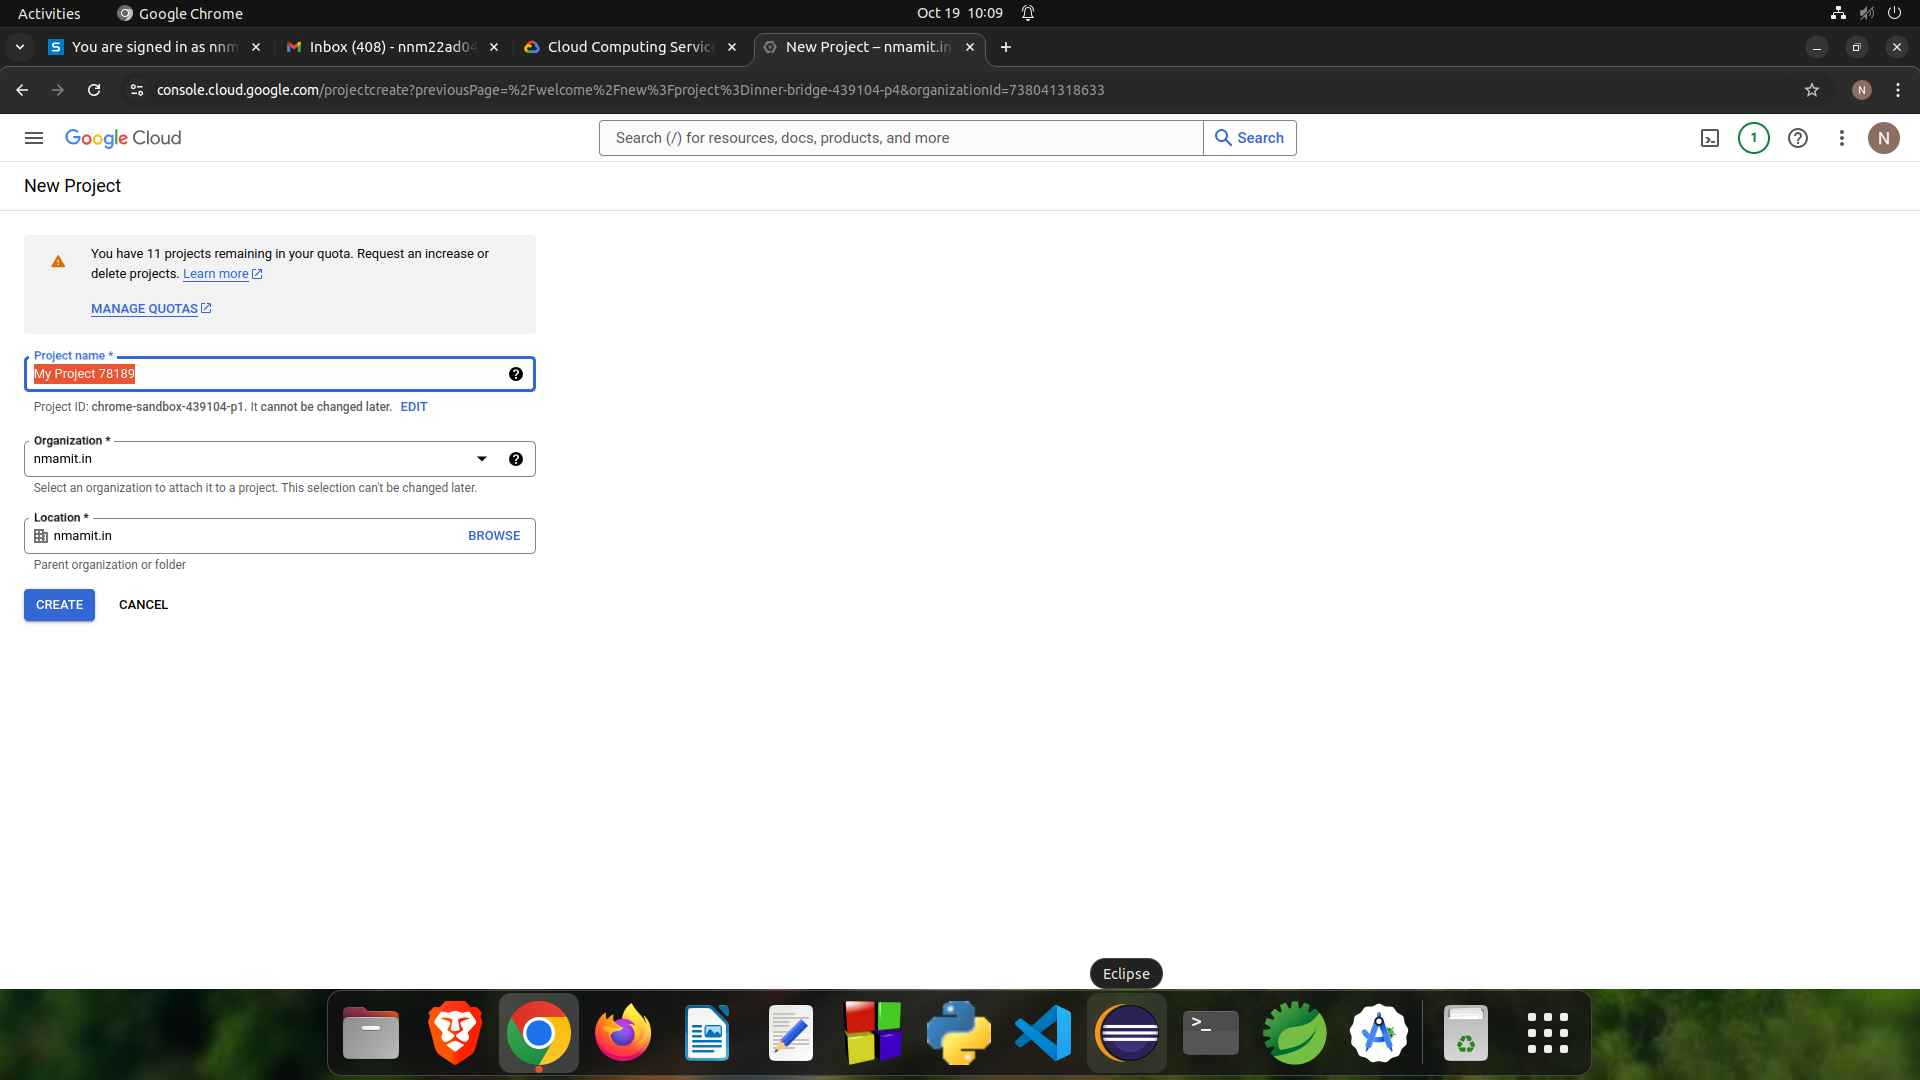
\includegraphics[width=0.6\textwidth]{exp 5/Screenshot from 2024-10-19 10-09-31.png}
    \caption{snapshot of creating a new project}
    \label{fig: 1}
\end{figure}

\begin{figure}[H]
    \centering
    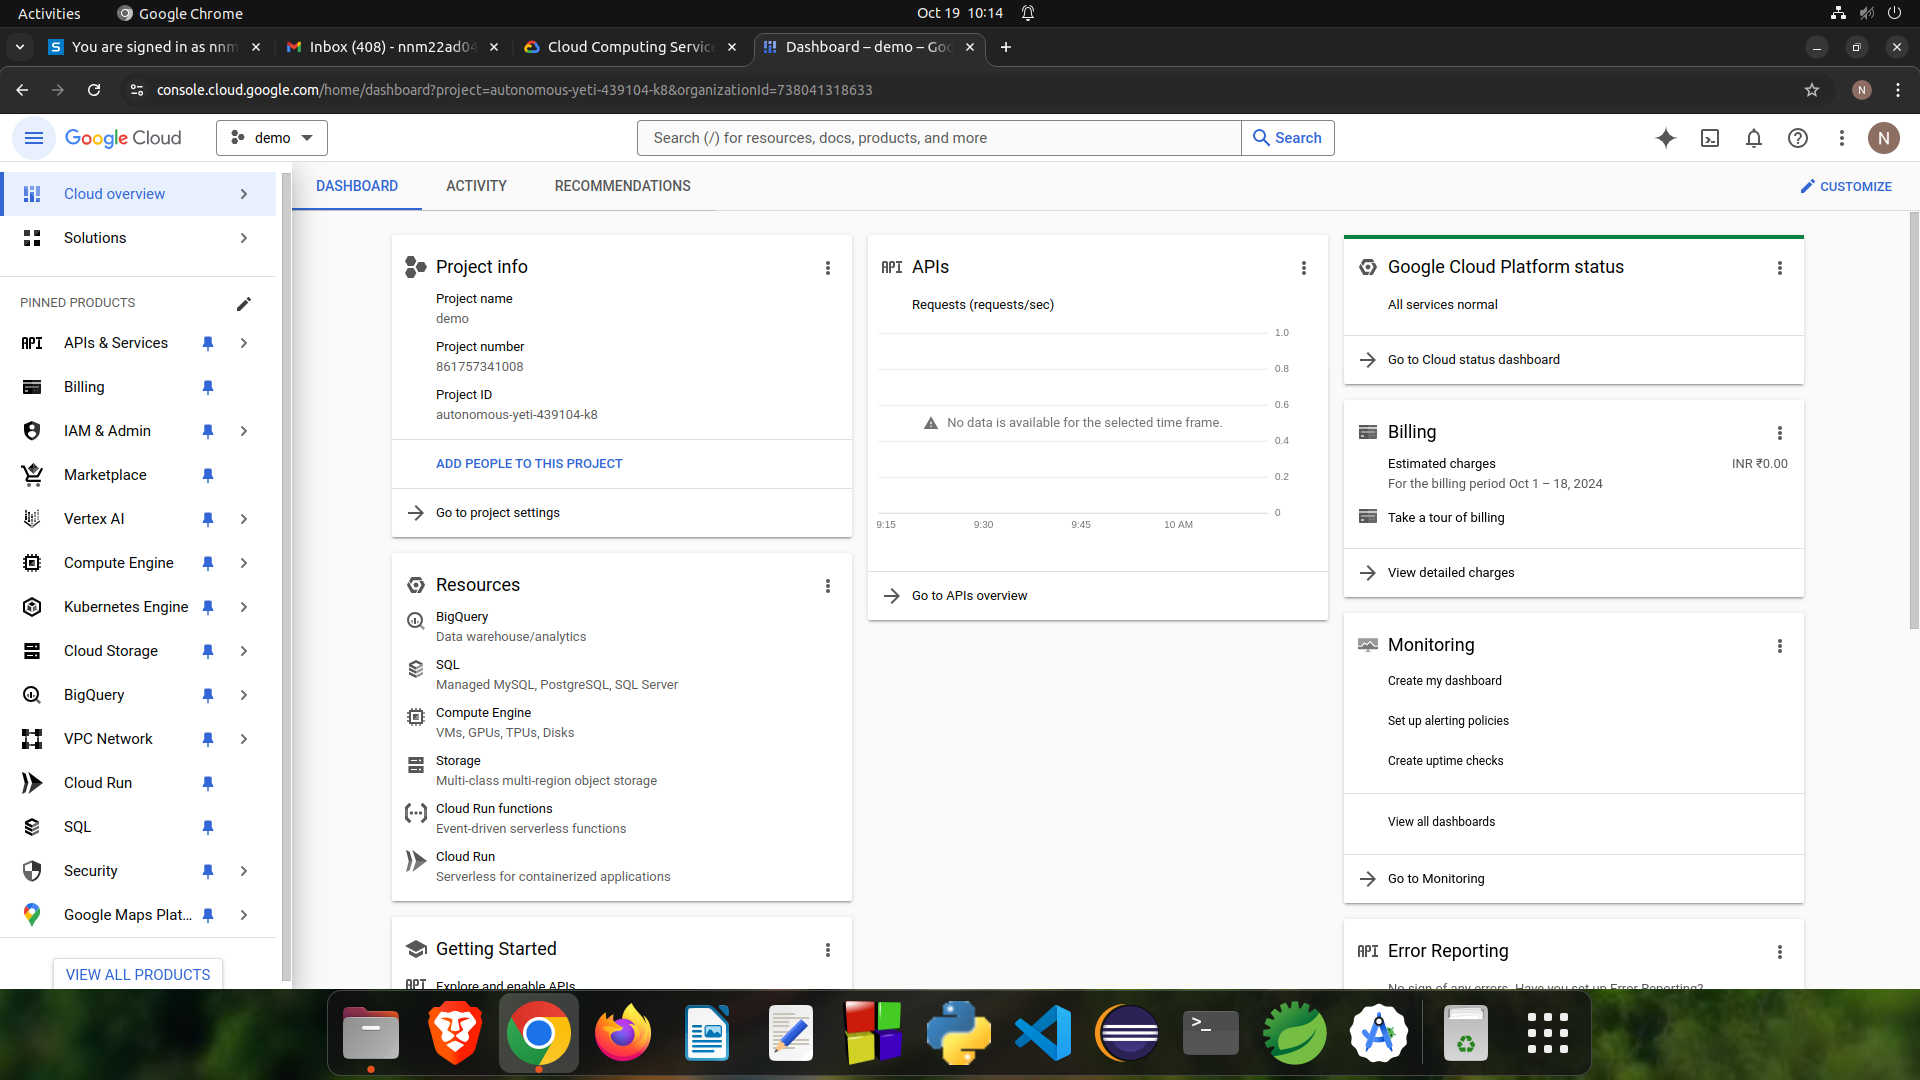
\includegraphics[width=0.8\textwidth]{exp 5/s5.png}
    \caption{Shows the project details - project ID}
    \label{fig: 1}
\end{figure}

\textbf{STEP 2:} \\
Navigate to the App Engine page to enable your application, select your project and click "Create Application," then choose an appropriate region for deployment. Next, proceed with Node.js installation if not already present on your system using the installation command.

\begin{center}
\texttt{sudo apt install npm}
\end{center}

\begin{figure}[H]
    \centering
    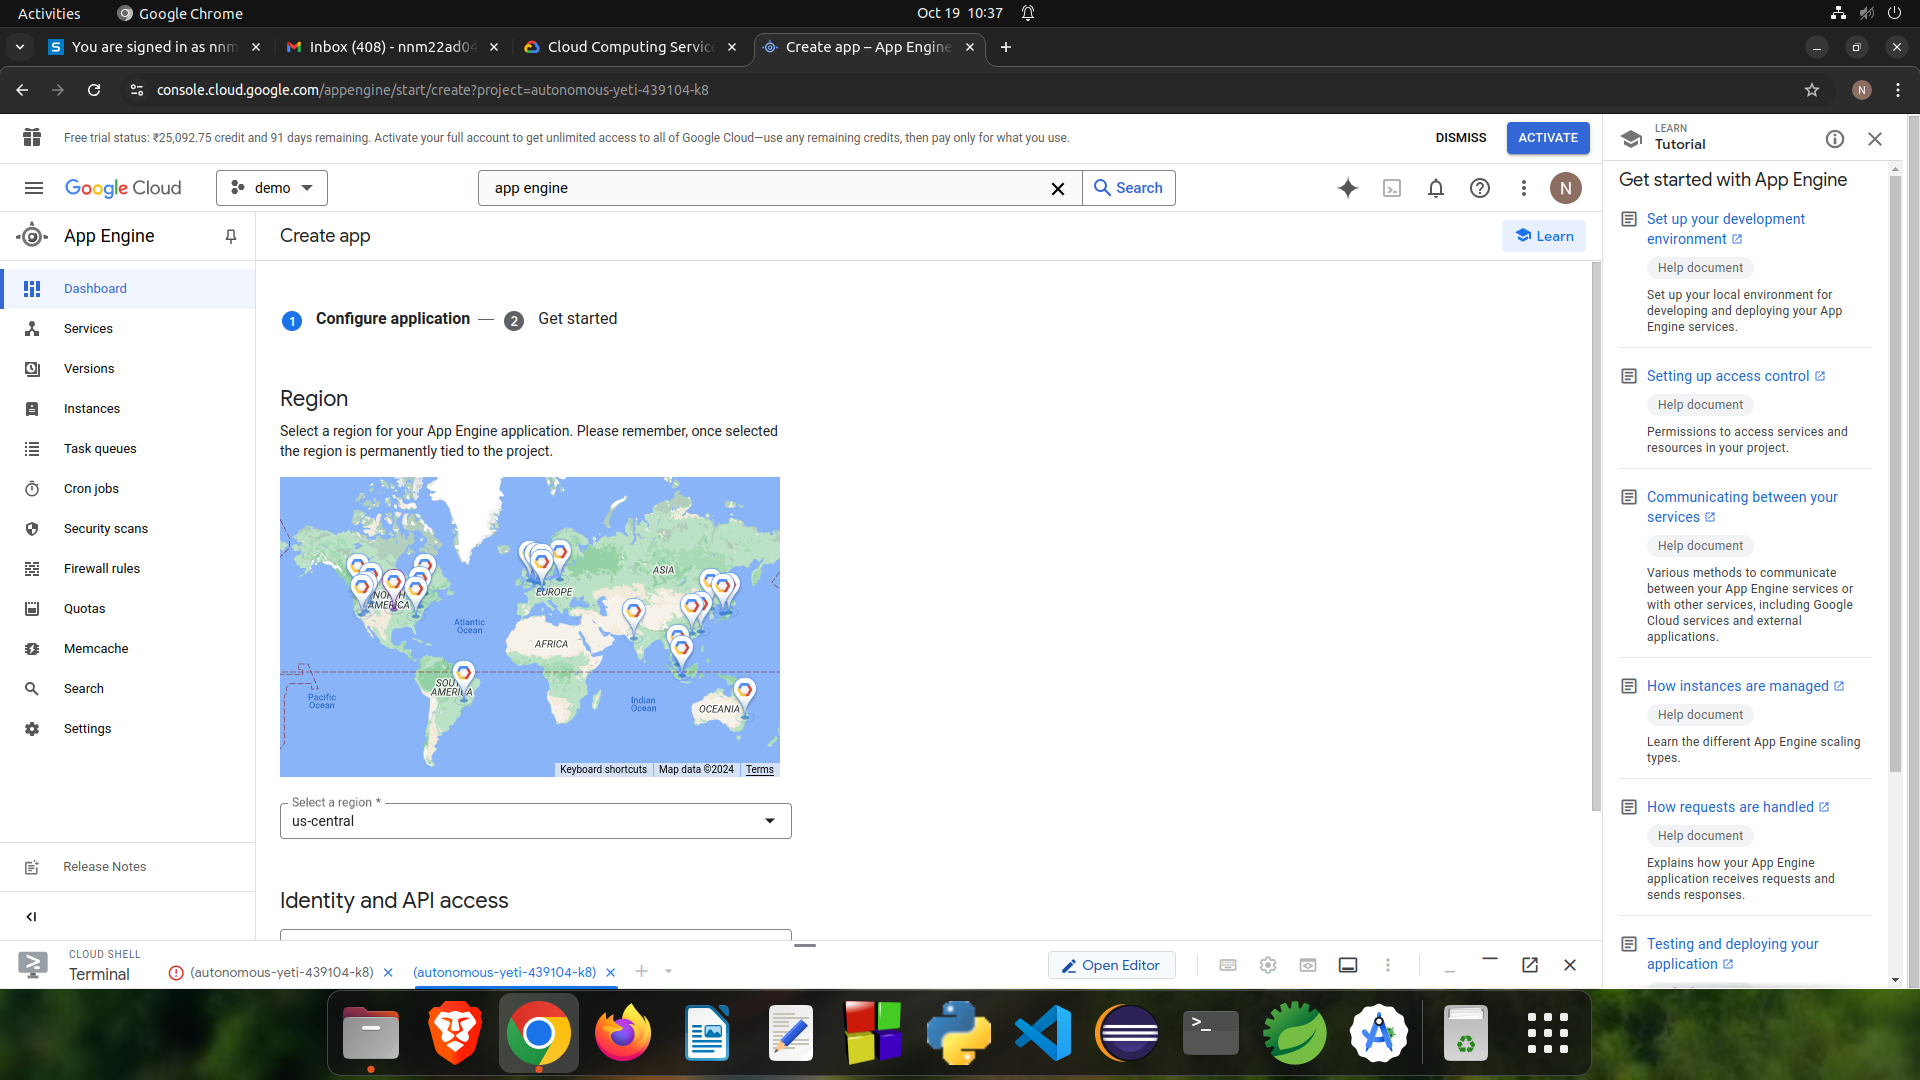
\includegraphics[width=0.8\textwidth]{exp 5/s10.png}
    \caption{Configure the app engine}
    \label{fig: 1}
\end{figure}

\begin{figure}[H]
    \centering
    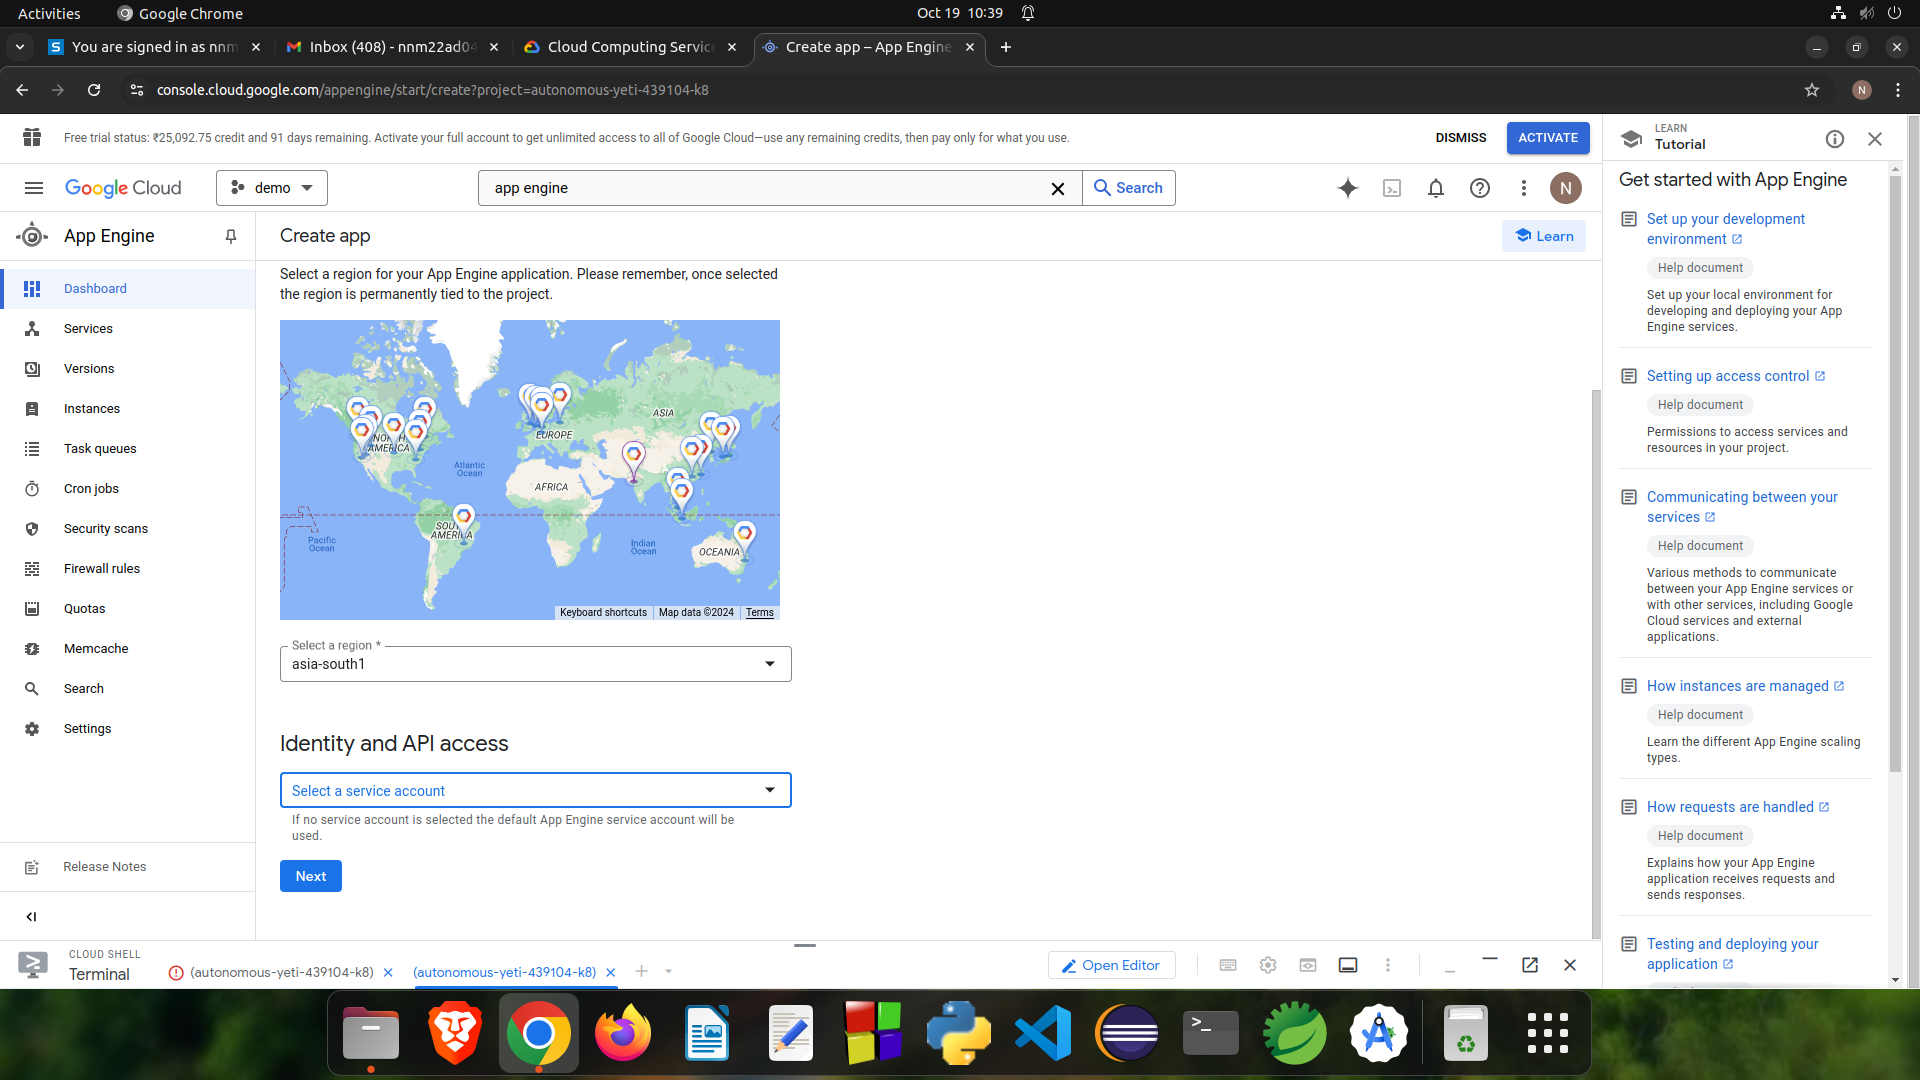
\includegraphics[width=0.8\textwidth]{exp 5/s11.png}
    \caption{Select the region}
    \label{fig: 1}
\end{figure}

\textbf{STEP 3:} \\
Initialize Google Cloud SDK, App Engine and Open the Terminal, Authenticate with Google Cloud:
\begin{itemize}
    \item Run the following command to log in:
    \begin{center}
    \texttt{gcloud auth login}
    \end{center}
\end{itemize}

\textbf{Set the Project:}
\begin{itemize}
    \item Set the project by running:
    \begin{center}
    \texttt{gcloud config set project YOUR\_PROJECT\_ID}
    \end{center}
\end{itemize}

\textbf{Initialize App Engine:}
\begin{itemize}
    \item Initialize App Engine by running:
    \begin{center}
    \texttt{gcloud app create project=YOUR\_PROJECT\_ID}
    \end{center}
\end{itemize}

\begin{figure}[H]
    \centering
    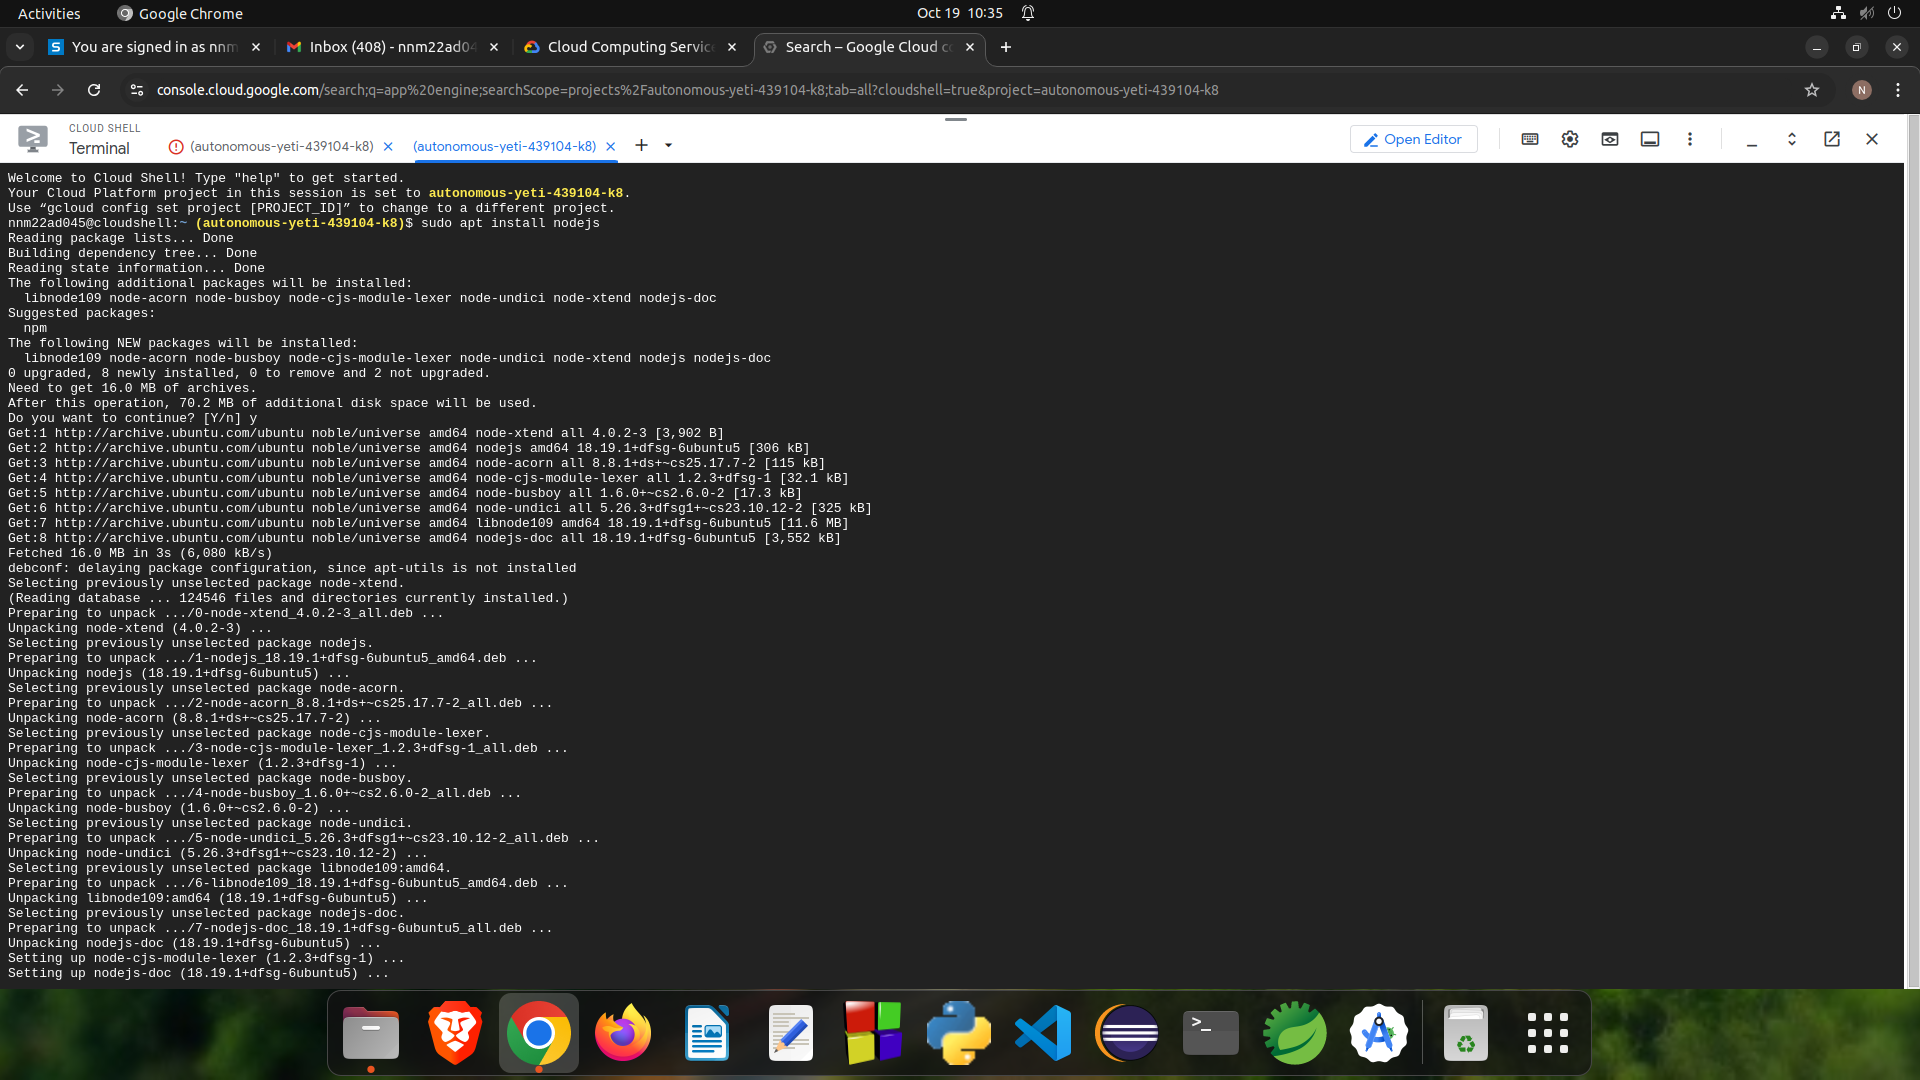
\includegraphics[width=0.8\textwidth]{exp 5/s9.png}
    \caption{Installing essential dependencies}
    \label{fig: 1}
\end{figure}

\textbf{Step 4: Create a Sample Node.js Application}

\textbf{1. Create a New Directory for Your Project:}
\begin{itemize}
    \item Create a directory called ‘hello-world-app‘ and navigate into it:
    \begin{center}
    \texttt{mkdir hello-world-app}
    \end{center}
    \begin{center}
    \texttt{cd hello-world-app}
    \end{center}
\end{itemize}

\textbf{2. Initialize the Node.js Project:}
\begin{itemize}
    \item Initialize the Node.js project by running:
    \begin{center}
    \texttt{npm init -y}
    \end{center}
\end{itemize}

\begin{figure}[H]
    \centering
    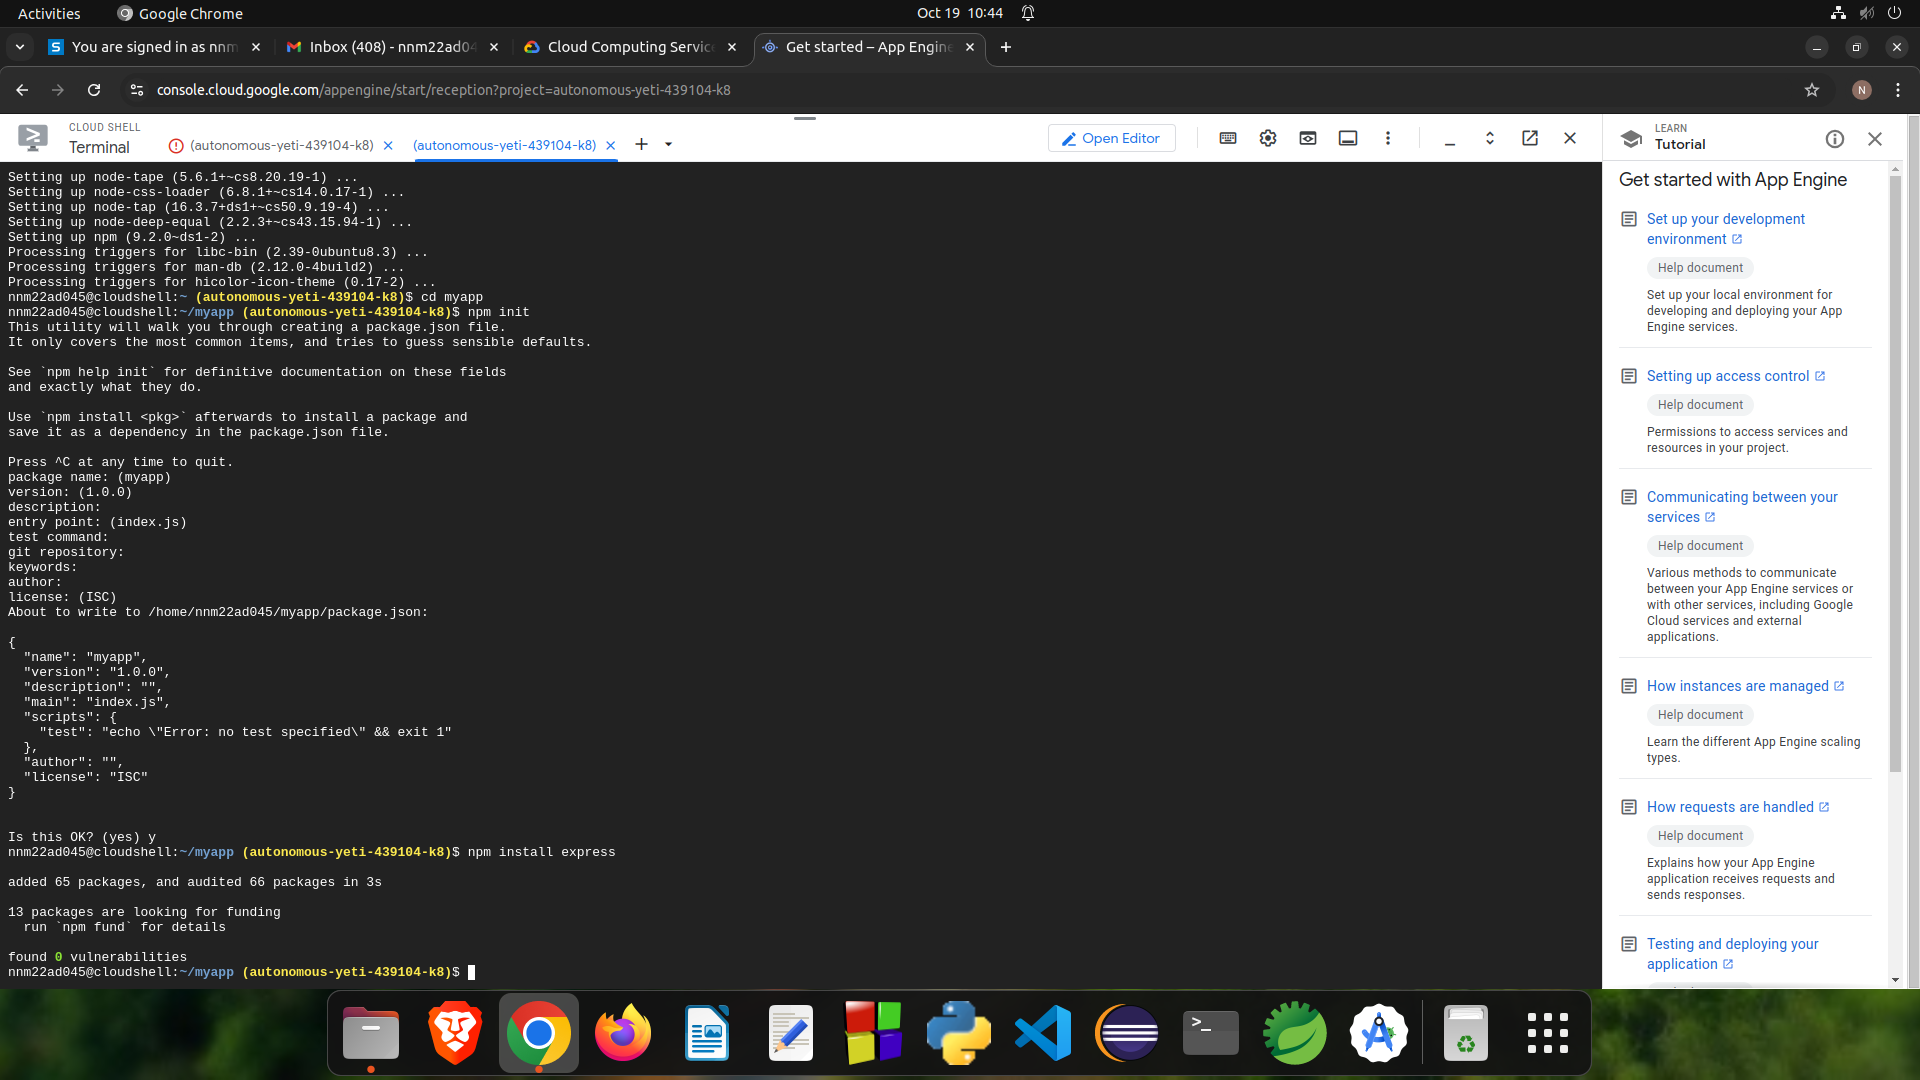
\includegraphics[width=0.8\textwidth]{exp 5/s16.png}
    \caption{Follow the setup instructions to set the application}
    \label{fig: 1}
\end{figure}

\textbf{3. Install Express:}
\begin{itemize}
    \item Install Express by running:
    \begin{center}
    \texttt{npm install express}
    \end{center}
\end{itemize}

\begin{figure}[H]
    \centering
    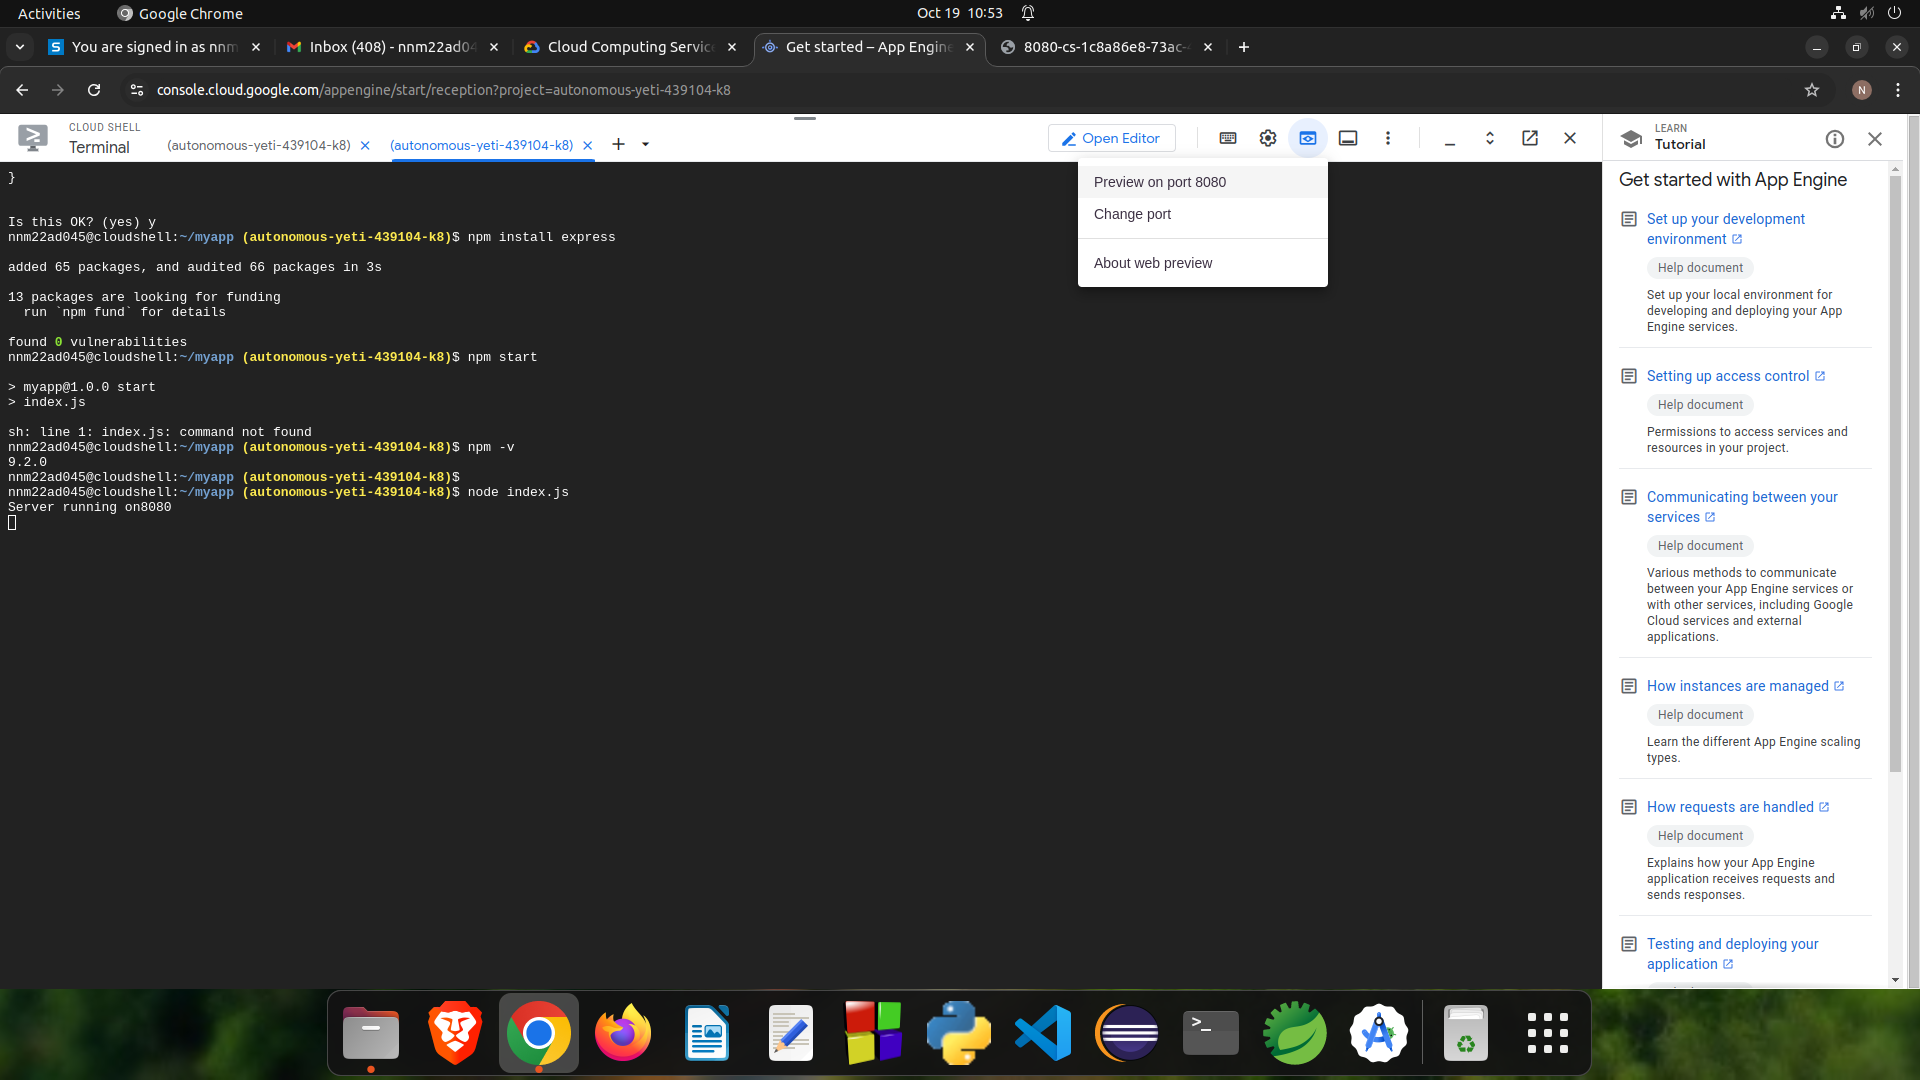
\includegraphics[width=0.8\textwidth]{exp 5/s20.png}
    \caption{Installing express}
    \label{fig: 1}
\end{figure}

\textbf{4. Create the Application:}
\begin{itemize}
    \item Create a file ‘index.js‘ and add the following code:
    \begin{center}
    \begin{verbatim}
const express = require('express');
const app = express();
const PORT = process.env.PORT || 8080;

app.get('/', (req, res) => {
  res.send("Hello World!");
});

app.listen(PORT, () => {
  console.log('Server is running on port ${PORT}');
});
    \end{verbatim}
    \end{center}
\end{itemize}

\begin{figure}[H]
    \centering
    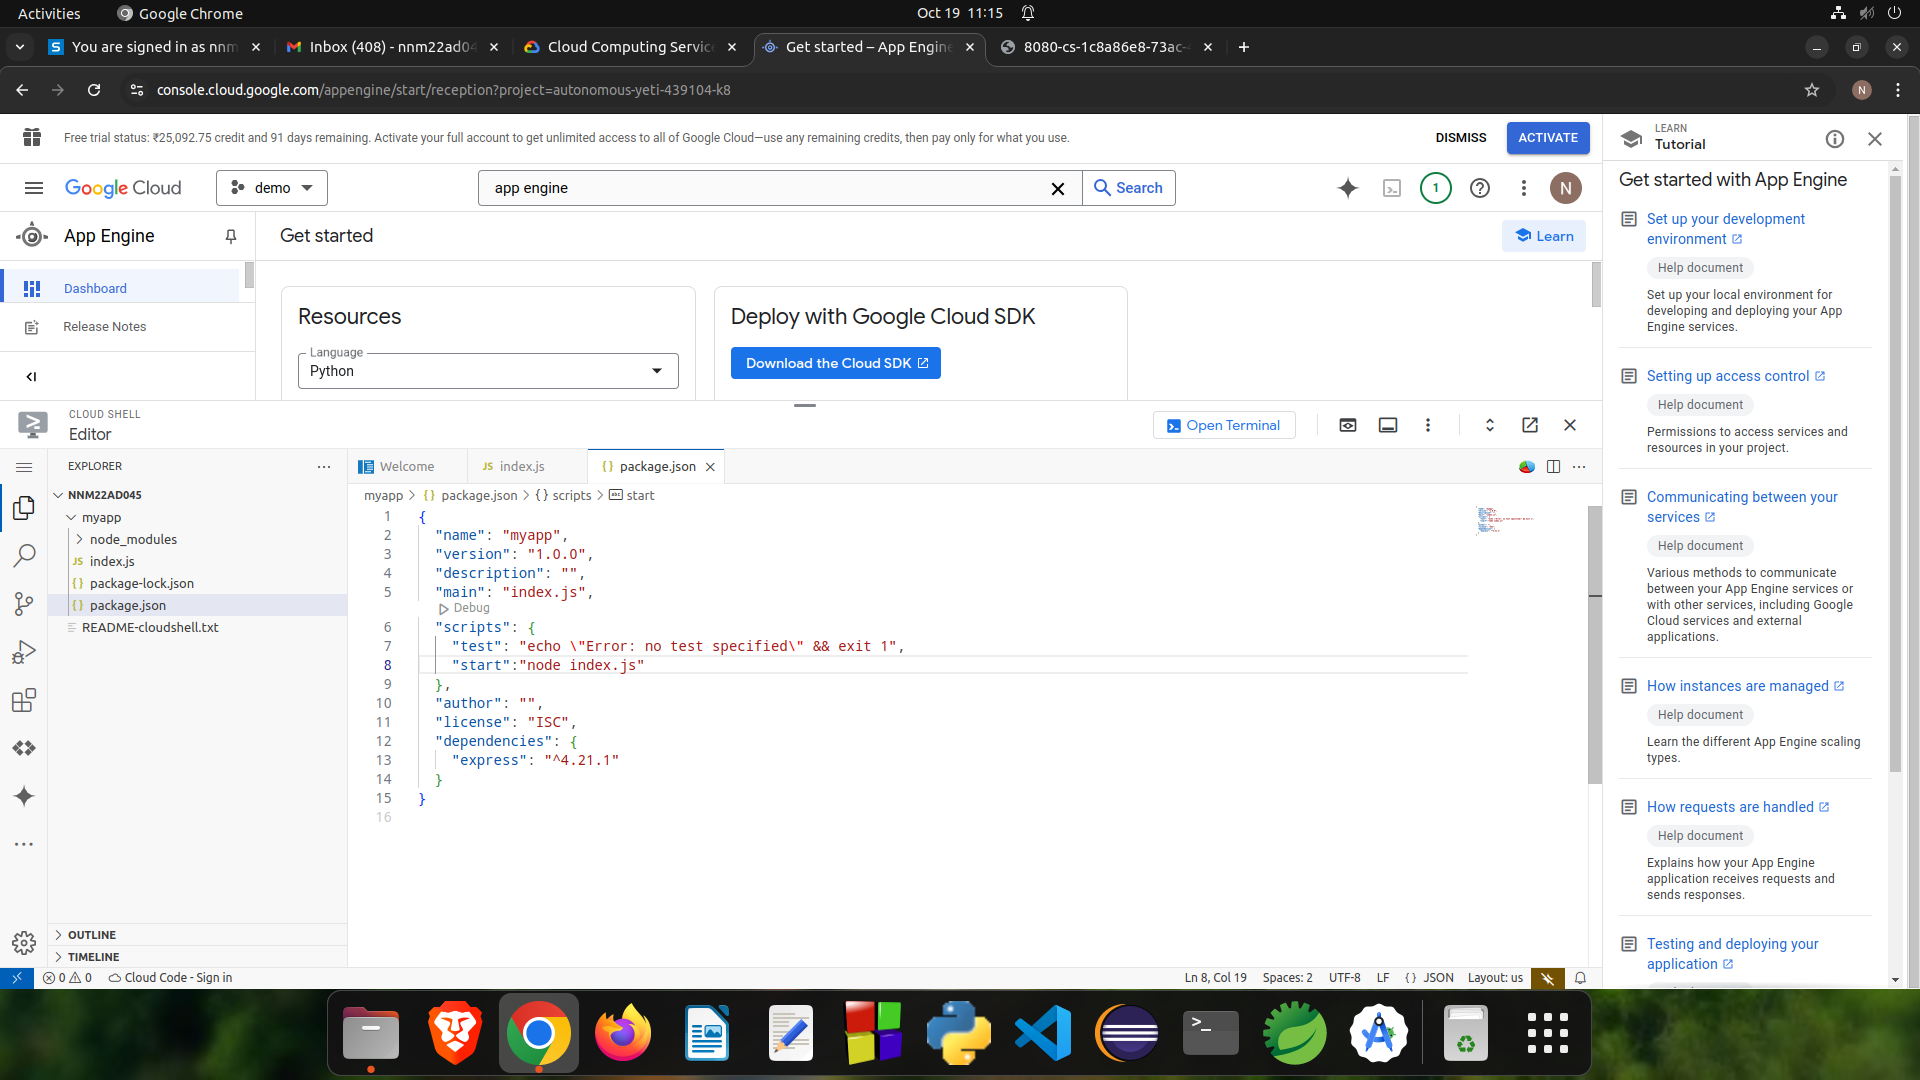
\includegraphics[width=0.8\textwidth]{exp 5/s22.png}
    \caption{Index.js hello world program}
    \label{fig: 1}
\end{figure}

\textbf{5. Create an app.yaml File:}
\begin{itemize}
    \item In the ‘hello-world-app‘ directory, create an ‘app.yaml‘ file with the following content:
    \begin{center}
    \begin{verbatim}
runtime: nodejs18
    \end{verbatim}
    \end{center}
\end{itemize}

\begin{figure}[H]
    \centering
    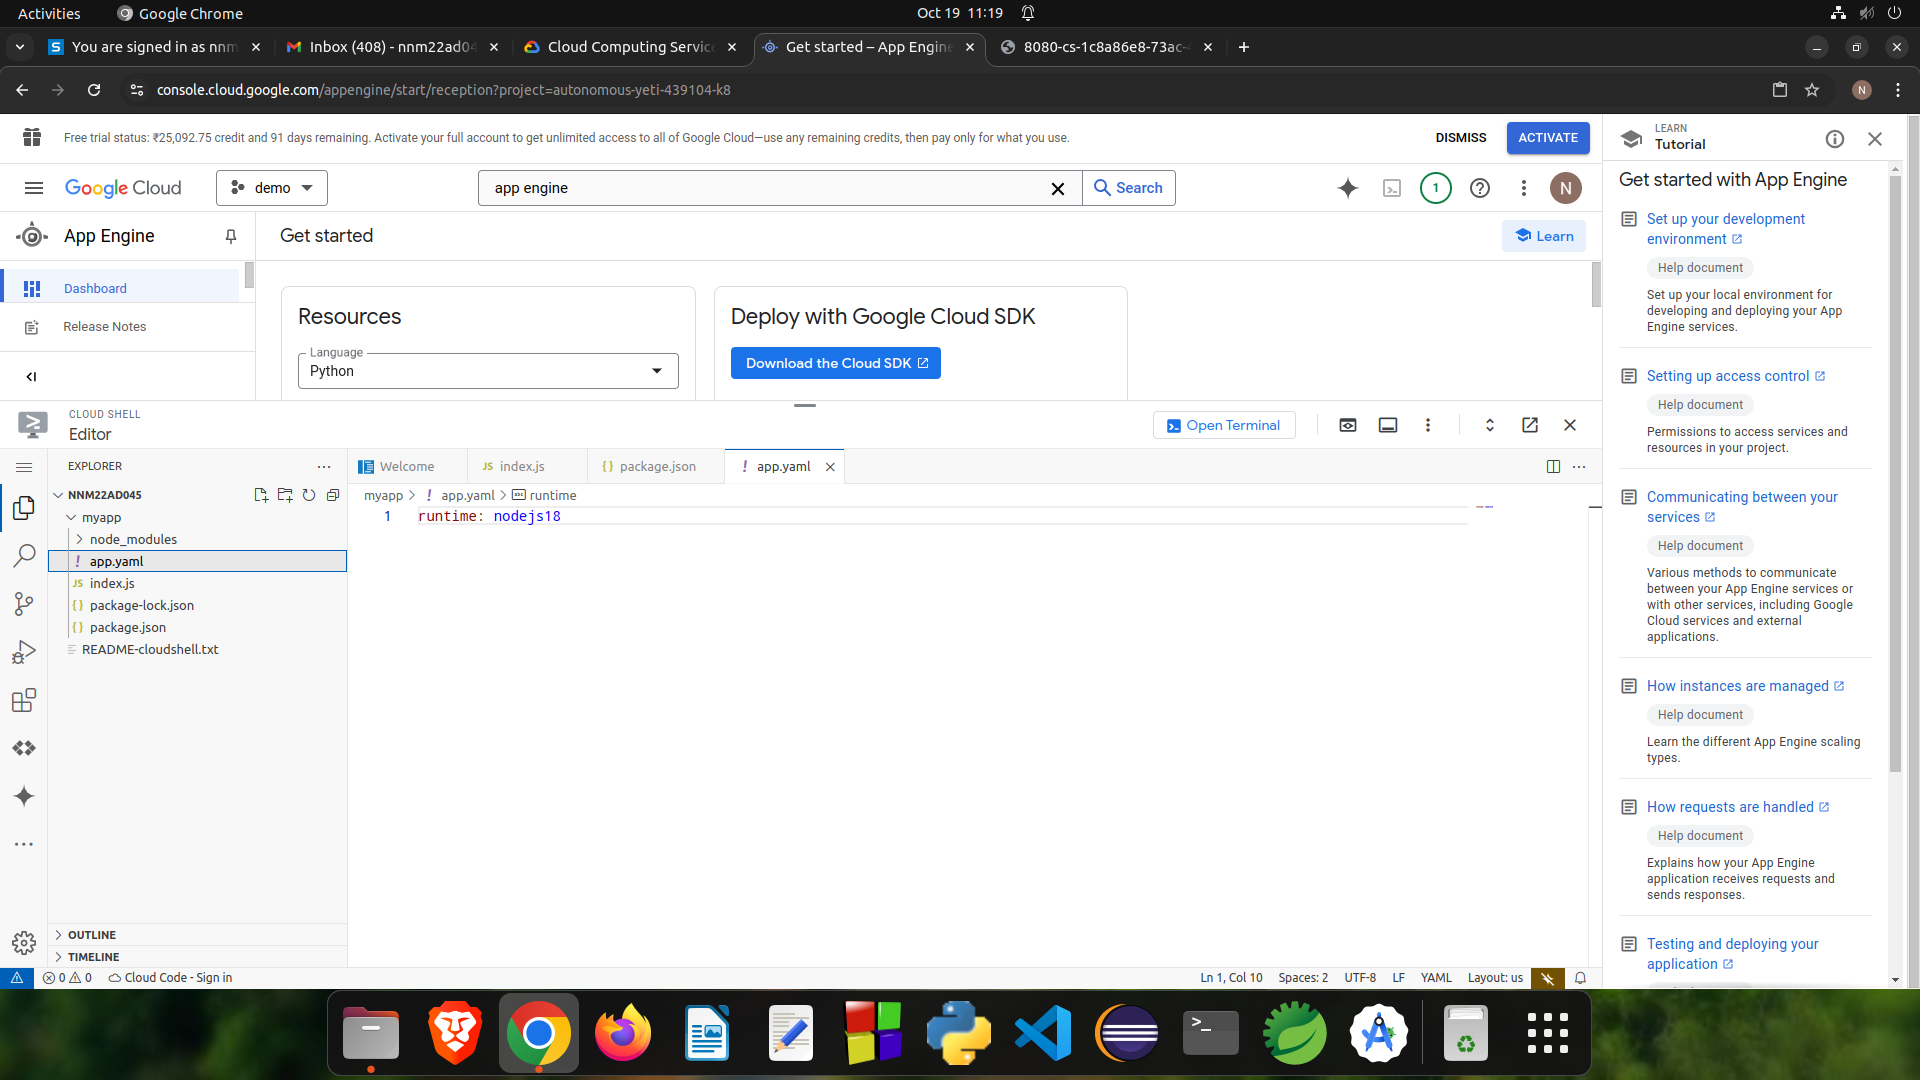
\includegraphics[width=0.8\textwidth]{exp 5/s23.png}
    \caption{Runtime nodejs 18}
    \label{fig: 1}
\end{figure}


\textbf{Step 5: Deploy to Google App Engine}

\textbf{1. Deploy the Application:}
\begin{itemize}
    \item Run the following command to deploy the application:
    \begin{center}
    \texttt{gcloud app deploy}
    \end{center}
\end{itemize}

\textbf{Step 6: Launch and Test the Application}

\textbf{1. Open the Application:}
\begin{itemize}
    \item Run the following command to open the application in the browser:
    \begin{center}
    \texttt{gcloud app browse}
    \end{center}
\end{itemize}

\begin{figure}[H]
    \centering
    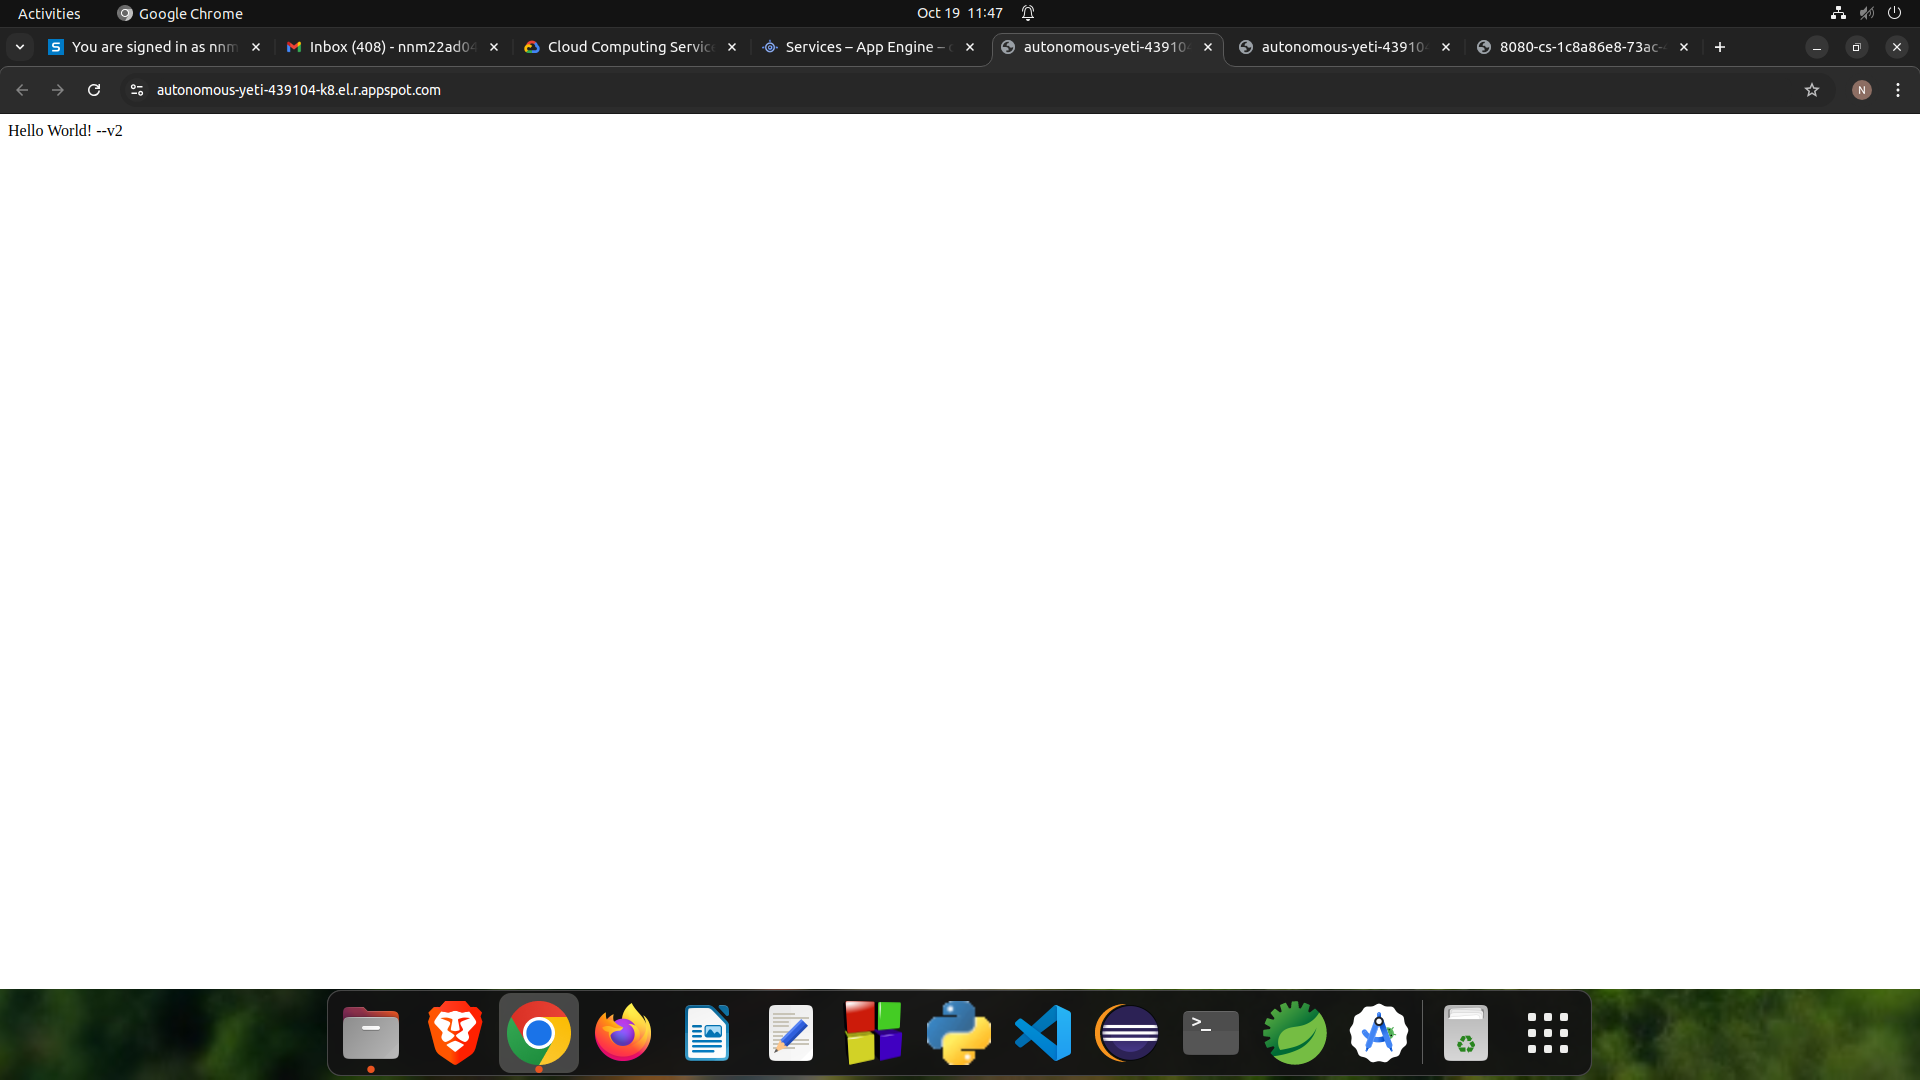
\includegraphics[width=0.8\textwidth]{exp 5/s35.png}
    \caption{Snapshot of the Output}
    \label{fig: 1}
\end{figure}

\subsection{Result} 
With these steps, the ”Hello World” application has been successfully deployed using
Google Cloud Platform’s PaaS (Google App Engine) with Node.js.


\newpage






\end{justify}
\end{adjustwidth}
\end{spacing}
\end{document}